%% bare_jrnl_compsoc.tex
%% V1.4a
%% 2014/09/17
%% by Michael Shell
%% See:
%% http://www.michaelshell.org/
%% for current contact information.
%%
%% This is a skeleton file demonstrating the use of IEEEtran.cls
%% (requires IEEEtran.cls version 1.8a or later) with an IEEE
%% Computer Society journal paper.
%%
%% Support sites:
%% http://www.michaelshell.org/tex/ieeetran/
%% http://www.ctan.org/tex-archive/macros/latex/contrib/IEEEtran/
%% and
%% http://www.ieee.org/

%%*************************************************************************
%% Legal Notice:
%% This code is offered as-is without any warranty either expressed or
%% implied; without even the implied warranty of MERCHANTABILITY or
%% FITNESS FOR A PARTICULAR PURPOSE! 
%% User assumes all risk.
%% In no event shall IEEE or any contributor to this code be liable for
%% any damages or losses, including, but not limited to, incidental,
%% consequential, or any other damages, resulting from the use or misuse
%% of any information contained here.
%%
%% All comments are the opinions of their respective authors and are not
%% necessarily endorsed by the IEEE.
%%
%% This work is distributed under the LaTeX Project Public License (LPPL)
%% ( http://www.latex-project.org/ ) version 1.3, and may be freely used,
%% distributed and modified. A copy of the LPPL, version 1.3, is included
%% in the base LaTeX documentation of all distributions of LaTeX released
%% 2003/12/01 or later.
%% Retain all contribution notices and credits.
%% ** Modified files should be clearly indicated as such, including  **
%% ** renaming them and changing author support contact information. **
%%
%% File list of work: IEEEtran.cls, IEEEtran_HOWTO.pdf, bare_adv.tex,
%%                    bare_conf.tex, bare_jrnl.tex, bare_conf_compsoc.tex,
%%                    bare_jrnl_compsoc.tex, bare_jrnl_transmag.tex
%%*************************************************************************


% *** Authors should verify (and, if needed, correct) their LaTeX system  ***
% *** with the testflow diagnostic prior to trusting their LaTeX platform ***
% *** with production work. IEEE's font choices and paper sizes can       ***
% *** trigger bugs that do not appear when using other class files.       ***
% The testflow support page is at:
% http://www.michaelshell.org/tex/testflow/


\documentclass[10pt,journal,compsoc]{IEEEtran}
%
% If IEEEtran.cls has not been installed into the LaTeX system files,
% manually specify the path to it like:
% \documentclass[10pt,journal,compsoc]{../sty/IEEEtran}





% Some very useful LaTeX packages include:
% (uncomment the ones you want to load)


% *** MISC UTILITY PACKAGES ***
%
%\usepackage{ifpdf}
% Heiko Oberdiek's ifpdf.sty is very useful if you need conditional
% compilation based on whether the output is pdf or dvi.
% usage:
% \ifpdf
%   % pdf code
% \else
%   % dvi code
% \fi
% The latest version of ifpdf.sty can be obtained from:
% http://www.ctan.org/tex-archive/macros/latex/contrib/oberdiek/
% Also, note that IEEEtran.cls V1.7 and later provides a builtin
% \ifCLASSINFOpdf conditional that works the same way.
% When switching from latex to pdflatex and vice-versa, the compiler may
% have to be run twice to clear warning/error messages.






% *** CITATION PACKAGES ***
%
\ifCLASSOPTIONcompsoc
  % IEEE Computer Society needs nocompress option
  % requires cite.sty v4.0 or later (November 2003)
  \usepackage[nocompress]{cite}
\else
  % normal IEEE
  \usepackage{cite}
\fi
% cite.sty was written by Donald Arseneau
% V1.6 and later of IEEEtran pre-defines the format of the cite.sty package
% \cite{} output to follow that of IEEE. Loading the cite package will
% result in citation numbers being automatically sorted and properly
% "compressed/ranged". e.g., [1], [9], [2], [7], [5], [6] without using
% cite.sty will become [1], [2], [5]--[7], [9] using cite.sty. cite.sty's
% \cite will automatically add leading space, if needed. Use cite.sty's
% noadjust option (cite.sty V3.8 and later) if you want to turn this off
% such as if a citation ever needs to be enclosed in parenthesis.
% cite.sty is already installed on most LaTeX systems. Be sure and use
% version 5.0 (2009-03-20) and later if using hyperref.sty.
% The latest version can be obtained at:
% http://www.ctan.org/tex-archive/macros/latex/contrib/cite/
% The documentation is contained in the cite.sty file itself.
%
% Note that some packages require special options to format as the Computer
% Society requires. In particular, Computer Society  papers do not use
% compressed citation ranges as is done in typical IEEE papers
% (e.g., [1]-[4]). Instead, they list every citation separately in order
% (e.g., [1], [2], [3], [4]). To get the latter we need to load the cite
% package with the nocompress option which is supported by cite.sty v4.0
% and later. Note also the use of a CLASSOPTION conditional provided by
% IEEEtran.cls V1.7 and later.


  


% *** GRAPHICS RELATED PACKAGES ***
%
\ifCLASSINFOpdf
  \usepackage[pdftex]{graphicx}
   \graphicspath{{figures/}}
  % declare the path(s) where your graphic files are
  % \graphicspath{{../pdf/}{../jpeg/}}
  % and their extensions so you won't have to specify these with
  % every instance of \includegraphics
  % \DeclareGraphicsExtensions{.pdf,.jpeg,.png}
\else
  % or other class option (dvipsone, dvipdf, if not using dvips). graphicx
  % will default to the driver specified in the system graphics.cfg if no
  % driver is specified.
  % \usepackage[dvips]{graphicx}
  % declare the path(s) where your graphic files are
  % \graphicspath{{../eps/}}
  % and their extensions so you won't have to specify these with
  % every instance of \includegraphics
  % \DeclareGraphicsExtensions{.eps}
\fi
% graphicx was written by David Carlisle and Sebastian Rahtz. It is
% required if you want graphics, photos, etc. graphicx.sty is already
% installed on most LaTeX systems. The latest version and documentation
% can be obtained at: 
% http://www.ctan.org/tex-archive/macros/latex/required/graphics/
% Another good source of documentation is "Using Imported Graphics in
% LaTeX2e" by Keith Reckdahl which can be found at:
% http://www.ctan.org/tex-archive/info/epslatex/
%
% latex, and pdflatex in dvi mode, support graphics in encapsulated
% postscript (.eps) format. pdflatex in pdf mode supports graphics
% in .pdf, .jpeg, .png and .mps (metapost) formats. Users should ensure
% that all non-photo figures use a vector format (.eps, .pdf, .mps) and
% not a bitmapped formats (.jpeg, .png). IEEE frowns on bitmapped formats
% which can result in "jaggedy"/blurry rendering of lines and letters as
% well as large increases in file sizes.
%
% You can find documentation about the pdfTeX application at:
% http://www.tug.org/applications/pdftex






% *** MATH PACKAGES ***
%
\usepackage[cmex10]{amsmath}
% A popular package from the American Mathematical Society that provides
% many useful and powerful commands for dealing with mathematics. If using
% it, be sure to load this package with the cmex10 option to ensure that
% only type 1 fonts will utilized at all point sizes. Without this option,
% it is possible that some math symbols, particularly those within
% footnotes, will be rendered in bitmap form which will result in a
% document that can not be IEEE Xplore compliant!
%
% Also, note that the amsmath package sets \interdisplaylinepenalty to 10000
% thus preventing page breaks from occurring within multiline equations. Use:
%\interdisplaylinepenalty=2500
% after loading amsmath to restore such page breaks as IEEEtran.cls normally
% does. amsmath.sty is already installed on most LaTeX systems. The latest
% version and documentation can be obtained at:
% http://www.ctan.org/tex-archive/macros/latex/required/amslatex/math/


\usepackage{amsfonts} % to use $\mathbb{Z}$


% *** SPECIALIZED LIST PACKAGES ***

\usepackage{algorithm}
\usepackage{algorithmic}
% algorithmic.sty was written by Peter Williams and Rogerio Brito.
% This package provides an algorithmic environment fo describing algorithms.
% You can use the algorithmic environment in-text or within a figure
% environment to provide for a floating algorithm. Do NOT use the algorithm
% floating environment provided by algorithm.sty (by the same authors) or
% algorithm2e.sty (by Christophe Fiorio) as IEEE does not use dedicated
% algorithm float types and packages that provide these will not provide
% correct IEEE style captions. The latest version and documentation of
% algorithmic.sty can be obtained at:
% http://www.ctan.org/tex-archive/macros/latex/contrib/algorithms/
% There is also a support site at:
% http://algorithms.berlios.de/index.html
% Also of interest may be the (relatively newer and more customizable)
% algorithmicx.sty package by Szasz Janos:
% http://www.ctan.org/tex-archive/macros/latex/contrib/algorithmicx/




% *** ALIGNMENT PACKAGES ***
%
%\usepackage{array}
% Frank Mittelbach's and David Carlisle's array.sty patches and improves
% the standard LaTeX2e array and tabular environments to provide better
% appearance and additional user controls. As the default LaTeX2e table
% generation code is lacking to the point of almost being broken with
% respect to the quality of the end results, all users are strongly
% advised to use an enhanced (at the very least that provided by array.sty)
% set of table tools. array.sty is already installed on most systems. The
% latest version and documentation can be obtained at:
% http://www.ctan.org/tex-archive/macros/latex/required/tools/


% IEEEtran contains the IEEEeqnarray family of commands that can be used to
% generate multiline equations as well as matrices, tables, etc., of high
% quality.




% *** SUBFIGURE PACKAGES ***
%\ifCLASSOPTIONcompsoc
%  \usepackage[caption=false,font=footnotesize,labelfont=sf,textfont=sf]{subfig}
%\else
%  \usepackage[caption=false,font=footnotesize]{subfig}
%\fi
% subfig.sty, written by Steven Douglas Cochran, is the modern replacement
% for subfigure.sty, the latter of which is no longer maintained and is
% incompatible with some LaTeX packages including fixltx2e. However,
% subfig.sty requires and automatically loads Axel Sommerfeldt's caption.sty
% which will override IEEEtran.cls' handling of captions and this will result
% in non-IEEE style figure/table captions. To prevent this problem, be sure
% and invoke subfig.sty's "caption=false" package option (available since
% subfig.sty version 1.3, 2005/06/28) as this is will preserve IEEEtran.cls
% handling of captions.
% Note that the Computer Society format requires a sans serif font rather
% than the serif font used in traditional IEEE formatting and thus the need
% to invoke different subfig.sty package options depending on whether
% compsoc mode has been enabled.
%
% The latest version and documentation of subfig.sty can be obtained at:
% http://www.ctan.org/tex-archive/macros/latex/contrib/subfig/




% *** FLOAT PACKAGES ***
%
%\usepackage{fixltx2e}
% fixltx2e, the successor to the earlier fix2col.sty, was written by
% Frank Mittelbach and David Carlisle. This package corrects a few problems
% in the LaTeX2e kernel, the most notable of which is that in current
% LaTeX2e releases, the ordering of single and double column floats is not
% guaranteed to be preserved. Thus, an unpatched LaTeX2e can allow a
% single column figure to be placed prior to an earlier double column
% figure. The latest version and documentation can be found at:
% http://www.ctan.org/tex-archive/macros/latex/base/


%\usepackage{stfloats}
% stfloats.sty was written by Sigitas Tolusis. This package gives LaTeX2e
% the ability to do double column floats at the bottom of the page as well
% as the top. (e.g., "\begin{figure*}[!b]" is not normally possible in
% LaTeX2e). It also provides a command:
%\fnbelowfloat
% to enable the placement of footnotes below bottom floats (the standard
% LaTeX2e kernel puts them above bottom floats). This is an invasive package
% which rewrites many portions of the LaTeX2e float routines. It may not work
% with other packages that modify the LaTeX2e float routines. The latest
% version and documentation can be obtained at:
% http://www.ctan.org/tex-archive/macros/latex/contrib/sttools/
% Do not use the stfloats baselinefloat ability as IEEE does not allow
% \baselineskip to stretch. Authors submitting work to the IEEE should note
% that IEEE rarely uses double column equations and that authors should try
% to avoid such use. Do not be tempted to use the cuted.sty or midfloat.sty
% packages (also by Sigitas Tolusis) as IEEE does not format its papers in
% such ways.
% Do not attempt to use stfloats with fixltx2e as they are incompatible.
% Instead, use Morten Hogholm'a dblfloatfix which combines the features
% of both fixltx2e and stfloats:
%
% \usepackage{dblfloatfix}
% The latest version can be found at:
% http://www.ctan.org/tex-archive/macros/latex/contrib/dblfloatfix/




%\ifCLASSOPTIONcaptionsoff
%  \usepackage[nomarkers]{endfloat}
% \let\MYoriglatexcaption\caption
% \renewcommand{\caption}[2][\relax]{\MYoriglatexcaption[#2]{#2}}
%\fi
% endfloat.sty was written by James Darrell McCauley, Jeff Goldberg and 
% Axel Sommerfeldt. This package may be useful when used in conjunction with 
% IEEEtran.cls'  captionsoff option. Some IEEE journals/societies require that
% submissions have lists of figures/tables at the end of the paper and that
% figures/tables without any captions are placed on a page by themselves at
% the end of the document. If needed, the draftcls IEEEtran class option or
% \CLASSINPUTbaselinestretch interface can be used to increase the line
% spacing as well. Be sure and use the nomarkers option of endfloat to
% prevent endfloat from "marking" where the figures would have been placed
% in the text. The two hack lines of code above are a slight modification of
% that suggested by in the endfloat docs (section 8.4.1) to ensure that
% the full captions always appear in the list of figures/tables - even if
% the user used the short optional argument of \caption[]{}.
% IEEE papers do not typically make use of \caption[]'s optional argument,
% so this should not be an issue. A similar trick can be used to disable
% captions of packages such as subfig.sty that lack options to turn off
% the subcaptions:
% For subfig.sty:
% \let\MYorigsubfloat\subfloat
% \renewcommand{\subfloat}[2][\relax]{\MYorigsubfloat[]{#2}}
% However, the above trick will not work if both optional arguments of
% the \subfloat command are used. Furthermore, there needs to be a
% description of each subfigure *somewhere* and endfloat does not add
% subfigure captions to its list of figures. Thus, the best approach is to
% avoid the use of subfigure captions (many IEEE journals avoid them anyway)
% and instead reference/explain all the subfigures within the main caption.
% The latest version of endfloat.sty and its documentation can obtained at:
% http://www.ctan.org/tex-archive/macros/latex/contrib/endfloat/
%
% The IEEEtran \ifCLASSOPTIONcaptionsoff conditional can also be used
% later in the document, say, to conditionally put the References on a 
% page by themselves.




% *** PDF, URL AND HYPERLINK PACKAGES ***
%
\usepackage{url}
% url.sty was written by Donald Arseneau. It provides better support for
% handling and breaking URLs. url.sty is already installed on most LaTeX
% systems. The latest version and documentation can be obtained at:
% http://www.ctan.org/tex-archive/macros/latex/contrib/url/
% Basically, \url{my_url_here}.





% *** Do not adjust lengths that control margins, column widths, etc. ***
% *** Do not use packages that alter fonts (such as pslatex).         ***
% There should be no need to do such things with IEEEtran.cls V1.6 and later.
% (Unless specifically asked to do so by the journal or conference you plan
% to submit to, of course. )


% correct bad hyphenation here
\hyphenation{op-tical net-works semi-conduc-tor  Birmingham}


\begin{document}
%
% paper title
% Titles are generally capitalized except for words such as a, an, and, as,
% at, but, by, for, in, nor, of, on, or, the, to and up, which are usually
% not capitalized unless they are the first or last word of the title.
% Linebreaks \\ can be used within to get better formatting as desired.
% Do not put math or special symbols in the title.
% \title{Bare Demo of IEEEtran.cls\\ for Computer Society Journals}
\title{Automatic Non-linear Analysis of the Variability of Human Activities}

%
%
% author names and IEEE memberships
% note positions of commas and nonbreaking spaces ( ~ ) LaTeX will not break
% a structure at a ~ so this keeps an author's name from being broken across
% two lines.
% use \thanks{} to gain access to the first footnote area
% a separate \thanks must be used for each paragraph as LaTeX2e's \thanks
% was not built to handle multiple paragraphs
%
%
%\IEEEcompsocitemizethanks is a special \thanks that produces the bulleted
% lists the Computer Society journals use for "first footnote" author
% affiliations. Use \IEEEcompsocthanksitem which works much like \item
% for each affiliation group. When not in compsoc mode,
% \IEEEcompsocitemizethanks becomes like \thanks and
% \IEEEcompsocthanksitem becomes a line break with idention. This
% facilitates dual compilation, although admittedly the differences in the
% desired content of \author between the different types of papers makes a
% one-size-fits-all approach a daunting prospect. For instance, compsoc 
% journal papers have the author affiliations above the "Manuscript
% received ..."  text while in non-compsoc journals this is reversed. Sigh.

\author{
Miguel~Xochicale,~\IEEEmembership{Doctoral~Researcher}\\

 \IEEEcompsocitemizethanks{\IEEEcompsocthanksitem 
 M. Xochicale is with the School of Electronic, Electrical and Systems Engineering, 
 The University of Birmingham, U.K. \protect\\
 % note need leading \protect in front of \\ to get a newline within \thanks as
 % \\ is fragile and will error, could use \hfil\break instead.
 E-mail: see http://mxochicale.github.io/
 }% <-this 


% 	Michael~Shell,~\IEEEmembership{Member,~IEEE,}
%         John~Doe,~\IEEEmembership{Fellow,~OSA,}
%         and~Jane~Doe,~\IEEEmembership{Life~Fellow,~IEEE}% <-this % stops a space
% \IEEEcompsocitemizethanks{\IEEEcompsocthanksitem M. Shell is with the Department
% of Electrical and Computer Engineering, Georgia Institute of Technology, Atlanta,
% GA, 30332.\protect\\
% % note need leading \protect in front of \\ to get a newline within \thanks as
% % \\ is fragile and will error, could use \hfil\break instead.
% E-mail: see http://www.michaelshell.org/contact.html
% \IEEEcompsocthanksitem J. Doe and J. Doe are with Anonymous University.}% <-this 
% stops an unwanted space
% \thanks{Manuscript received April 19, 2005; revised September 17, 2014.}
}

% note the % following the last \IEEEmembership and also \thanks - 
% these prevent an unwanted space from occurring between the last author name
% and the end of the author line. i.e., if you had this:
% 
% \author{....lastname \thanks{...} \thanks{...} }
%                     ^------------^------------^----Do not want these spaces!
%
% a space would be appended to the last name and could cause every name on that
% line to be shifted left slightly. This is one of those "LaTeX things". For
% instance, "\textbf{A} \textbf{B}" will typeset as "A B" not "AB". To get
% "AB" then you have to do: "\textbf{A}\textbf{B}"
% \thanks is no different in this regard, so shield the last } of each \thanks
% that ends a line with a % and do not let a space in before the next \thanks.
% Spaces after \IEEEmembership other than the last one are OK (and needed) as
% you are supposed to have spaces between the names. For what it is worth,
% this is a minor point as most people would not even notice if the said evil
% space somehow managed to creep in.

% The paper headers
\markboth{Ninth Month Report, August~2015}%
{Shell \MakeLowercase{\textit{et al.}}: Bare Demo of IEEEtran.cls for Computer 
Society Journals}
% The only time the second header will appear is for the odd numbered pages
% after the title page when using the twoside option.
% 
% *** Note that you probably will NOT want to include the author's ***
% *** name in the headers of peer review papers.                   ***
% You can use \ifCLASSOPTIONpeerreview for conditional compilation here if
% you desire.

% The publisher's ID mark at the bottom of the page is less important with
% Computer Society journal papers as those publications place the marks
% outside of the main text columns and, therefore, unlike regular IEEE
% journals, the available text space is not reduced by their presence.
% If you want to put a publisher's ID mark on the page you can do it like
% this:
%\IEEEpubid{0000--0000/00\$00.00~\copyright~2014 IEEE}
% or like this to get the Computer Society new two part style.
%\IEEEpubid{\makebox[\columnwidth]{\hfill 0000--0000/00/\$00.00~\copyright~2014 IEEE}%
%\hspace{\columnsep}\makebox[\columnwidth]{Published by the IEEE Computer Society\hfill}}
% Remember, if you use this you must call \IEEEpubidadjcol in the second
% column for its text to clear the IEEEpubid mark (Computer Society jorunal
% papers don't need this extra clearance.)

% use for special paper notices
%\IEEEspecialpapernotice{(Invited Paper)}

% for Computer Society papers, we must declare the abstract and index terms
% PRIOR to the title within the \IEEEtitleabstractindextext IEEEtran
% command as these need to go into the title area created by \maketitle.
% As a general rule, do not put math, special symbols or citations
% in the abstract or keywords.
\IEEEtitleabstractindextext{%

\begin{abstract}
This report presents the progress for the 9 Month Report 
of the PhD research project titled
 ``Automatic Non-linear Analysis of the Variability of Human Activities``.
The PhD research project is aimed to explore and propose methods which help us 
to automatically identify the variability of human activities. 
In this report I particularly explored the use of time-delay
embedding and PCA methods as a metric for the variability of human activities.
I also reviewed the main components of the activity recognition chain
and presented the use of artificial signal to model the variability of human body activities.
I used salsa dancing activities as a case of study in order 
to apply time-delay embedding and PCA methods for which 
2-D reconstructed state spaces showed different shapes 
that were visually linked to the experience level of the participants.
Addiotionally, I present a publication plan and future work.
\end{abstract}




% Note that keywords are not normally used for peerreview papers.
\begin{IEEEkeywords}
Activity Recognition; On-Body Inertial Sensors; Motor Skill Assessment;
\end{IEEEkeywords}}


% make the title area
\maketitle


% To allow for easy dual compilation without having to reenter the
% abstract/keywords data, the \IEEEtitleabstractindextext text will
% not be used in maketitle, but will appear (i.e., to be "transported")
% here as \IEEEdisplaynontitleabstractindextext when the compsoc 
% or transmag modes are not selected <OR> if conference mode is selected 
% - because all conference papers position the abstract like regular
% papers do.
\IEEEdisplaynontitleabstractindextext
% \IEEEdisplaynontitleabstractindextext has no effect when using
% compsoc or transmag under a non-conference mode.



% For peer review papers, you can put extra information on the cover
% page as needed:
% \ifCLASSOPTIONpeerreview
% \begin{center} \bfseries EDICS Category: 3-BBND \end{center}
% \fi
%
% For peerreview papers, this IEEEtran command inserts a page break and
% creates the second title. It will be ignored for other modes.
\IEEEpeerreviewmaketitle



\IEEEraisesectionheading{\section{Introduction}\label{sec:introduction}}
% Computer Society journal (but not conference!) papers do something unusual
% with the very first section heading (almost always called "Introduction").
% They place it ABOVE the main text! IEEEtran.cls does not automatically do
% this for you, but you can achieve this effect with the provided
% \IEEEraisesectionheading{} command. Note the need to keep any \label that
% is to refer to the section immediately after \section in the above as
% \IEEEraisesectionheading puts \section within a raised box.

% The very first letter is a 2 line initial drop letter followed
% by the rest of the first word in caps (small caps for compsoc).
% 
% form to use if the first word consists of a single letter:
% \IEEEPARstart{A}{demo} file is ....
% 
% form to use if you need the single drop letter followed by
% normal text (unknown if ever used by IEEE):
% \IEEEPARstart{A}{}demo file is ....
% 
% Some journals put the first two words in caps:
% \IEEEPARstart{T}{his demo} file is ....
% 
% Here we have the typical use of a "T" for an initial drop letter
% and "HIS" in caps to complete the first word.




\IEEEPARstart{H}{uman} Activity Recognition (HAR) using body-worn sensors 
has been a topic of research for the last 20 years \cite{bulling2014, Lara2013}. 
This is due to three factors: (i) technology advances in sensors, 
(ii) longer battery lifetimes and (iii) different application-oriented scenarios.
The challenges of HAR are based on the complexity and diversity of human activities 
(e.g. ambulation, transportation, phone usage, daily activities, exercise, military);
the selection of different sensors to use (e.g. inertial, light, temperature or audio sensors)
\cite{Lara2013} and different bodily locations for sensor placement 
(e.g. chest, wrist, lower back, hip, thigh, foot) \cite{Cleland2013}.
This complexity and diversity results in a large number of options for 
configurations \cite{Mannini2013}.


According to Bulling \textit{et al.} \cite{bulling2014} the common challenges in HAR
using body-worn sensors are: 
(i) \textit{intraclass variability} which occurs when an activity is performed differently 
either by a single person or several people. For example, gait patterns may be more
dynamic in the morning after sleep than in the evening after a day full of activities; 
(ii) \textit{interclass similarity} occurs when the sensor data is very similar. For example,
recognising dietary activity, drinking water or coffee would entail the same arm movements 
\cite{amft2008phd}; and (iii) \textit{the NULL class problem} occurs 
when ambiguous activities are irrelevant for the recognition methods
which leads to wrong classification of the activities \cite{amft2011}.
Recently, Bulling \textit{et al.} \cite{bulling2014} reviewed advances in the Activity
Recognition Chain (ARC) using body-worn sensors. The general ARC comprises five stages
(data acquisition, signal processing, segmentation, feature extraction, and selection
training and classification) of which the applied technique in each stage depends on the
activity to recognise.


Activity recognition often seeks to treat variability and 
similarity as variations of the same problem, i.e., defining 
an ambiguous model of the activity to enable consistent
classification and recognition. By defining the model 
with sufficient clarity, it should be possible to reliably spot 
instances of the activity and to distinguish this from others
similar activities. The challenge faced by this PhD project 
is that identifying a specific instance will not be sufficient
to address the core question of how well is an action being performed?
Thus, rather than asking whether a dance step is being performed,
the question is whether this step is being made by an expert or a novice,
and more importantly, is the novice showing improvement from 
previous attempts. This 
also means that, rather than trying to reduce or design out
variability in the signal that is used for activity recognition,
this PhD is looking for ways to model and work with such
variability.


Therefore, the variability of dance activities is a very rich 
case of study to explore and investigate human 
movement variability. Variability is presented in either dance 
features (e.g. fluency of motion, coordination, steadiness of 
the rhythm, adding erratic or additional movements \cite{Grammer2011, Aristidou2014}) 
or some biological and demographic features of dancers 
(e.g. gender, age, home country \cite{Grammer2011, Iwai2011}). 

Hammerla \textit{et al.} \cite{hammerla2011} have examined the effects of
variability of motor performance using artificial signals so as 
to create motion structures (strategy of the motion activity) 
and motion noise (the precision of the motion) of human 
activities. To quantify the variability of motion activities, 
Hammerla \textit{et al.} \cite{hammerla2011} proposed the use of PCA to compute 
the area underneath the curve of the cumulative principal 
components which is used as a metric for motor skill assessment.
The variability in human activities has therefore 
a relation with quantitative assessment of motion structures 
and motion noise of human activities. 
Velloso \textit{et al.} \cite{Velloso2013a, Velloso2013b},
for example, assessed automatically the quality of weight-lifting 
activity to quantify how \textit{good} the repetition of 
weight-lifting activity is in terms of angles variation of each bone 
in relation to reference planes. 

The understanding of human behaviour using non-linear 
analysis has proven to make good advances since the early 1980s 
\cite{Huys2011, KantzSchreiber04}. For instance, concepts such as fractal 
dimensionality, the Lyapunov exponent or time-delay 
embedding have been applied to better understand the 
variability of human activities. Yamamoto \textit{et al.} \cite{Suzuki2013, Yamamoto2000} 
used the fractal dimensionality of an attractor 
(i.e. values that are close enough in the time-delay embedding)
to model repeated forehand and backhand tennis strokes.
Gouwanda \textit{et al.} \cite{Gouwanda2012} showed that the variability in walking 
speed has a linear relationship with the Lyapunov exponent. 
This exponent is an average of the natural logarithm of all 
the distances from the time-delay embedding and its nearest 
neighbour state space. Lyapunov exponent therefore is suitable
for analysing the temporal variation in gait stability.
The time-delay embedding has been used as a feature for 
general gait recognition \cite{Sama2013} as well as for recognition 
of cycling, running, walking upstairs and downstairs activities \cite{Frank2010}.
Recently,  Caballero \textit{et al.} \cite{Caballero2014} reviewed further non-linear 
analysis tools (e.g. local dynamic stability, recurrent quantification analysis, 
entropy measurements, detrended fluctuation analysis) to measure human movement 
variability.  However, the questions to ask, as pointed out by 
Caballero \textit{et al.} \cite{Caballero2014}, are: ``...do these tools actually 
measure variability?'' and ``what kind of variability?''.
It should be noted that non-linear analysis offers a range of techniques 
for the study of human activity (see \cite{Guastello2011} 
for an overview of alternative techniques). 

Given the case of the variability in dance activities, it is hypothesised that 
there are three possible reasons for variation:
(i) inherent noise in body-worn sensors, 
(ii) inherent properties of the activity itself and
(iii) differences in the people performing the activity, e.g., gender, 
anthropometry or level of skills.

\subsection{Research Questions}
For this PhD, the time-delay embedding and PCA methods
have proven to be a reliable method for feature extraction in HAR
\cite{Gouwanda2012, Sama2013, Frank2010}. It this therefore hypothesised that 
these methods might be suitable to learn the variability of human
activities. Therefore, the following research questions will be addressed:
\begin{enumerate}
\item How can the time-delay embedding and PCA methods quantify 
 the possible reasons of the variability of dance activities ?
\item In the light of limitations of time-delay embedding and PCA,
 which other non-linear analysis tools would be suitable to explore 
 the variability in different human activities and use them as a 
features for machine learning algorithms?
\item What is the best set of features that can yield the best recognition
rate of particular type of activity?
\item How does the sensor positioning influence the outcomes?
\item How can the expertise of the dancer be employed as a tool to empower
the design strategy?
\end{enumerate}




\section{Recognising Dexterity In Dance }
As Miura \textit{et al.} \cite{Miura2015} point out 
`` $\ldots$ how the human motor 
system produces dance movements is still poorly understood.''
Miura et al. \cite{Miura2013} measured muscle activation using 
electromyographic (EMG) data collected from muscles in 
the lower limb, for a task requiring participants to 
bounce up and down in time to a metronome beat. They 
demonstrated that experienced dancers show much better 
precision in synchronising  movements to beat than non-dancers, 
i.e., dancers maintained much lower standard deviation in 
temporal deviation against the beat than non-dancers. 
This result is consistent with work which shows that, compared with inexperienced- or 
non-dancers, trained ballet dancers exhibit superior postural 
stability \cite{Crotts1996}, and show superior ability in position matching 
of upper limbs \cite{Ramsay2001}.

Capturing dance activity through sensors has tended 
to rely on motion capture \cite{Alexiadis2014} or sensors mounted on the 
person \cite{Lynch2005} or in their shoes \cite{Paradiso1997} or data recorded from their 
smart phones \cite{Wei2014}. Much of this work has been concerned 
with using the dancers' motion to work with multimedia 
presentations that augment and complement the dance \cite{Griffith1998, Park2006}
or as interfacing with a game \cite{Chu2012} or commercial games, 
such as Dance Revolution. While the range of sensing 
technology used in these papers is diverse and the results 
of the activity recognition are varied, it is fair to say that 
few of the papers have considered variability  in how a 
dance is performed. In their work, Aristidou \textit{et al.} \cite{Aristidou2014} have 
considered the manner in which dance steps conform to 
a set of defined templates that describe steps in terms of 
a three-dimensional rotation (described using quaternions).  
The implication is that a goodness-of-fit can be ascertained 
to determine how good a dancer performs a step, and how 
any deviation from ‘good’ can be modified and improved 
through practice. 

For this report, we are interested in the question of how 
time-delay embedding and PCA techniques can provide 
insight into the variability and dexterity of dancers. To this 
end, we consider the performance of a set of steps from Salsa 
dance  as well as other dance styles in future and compare 
untrained, inexperienced or non-dancers in one cohort with 
experienced dancers in another.

Before explaining how the activity recognition chain, the next 
section outlines the approach to time-delay embedding and 
the resulting phase space representation used in this report. 



\section{Time-Delay Embedding}
The aim of time-delay embedding, also known as Takens's 
Theorem \cite{Takens1981}, is to reconstruct a $k-$dimensional manifold $M$ 
of an unknown dynamical system $s(t)$ from a time series 
$x(t)$ with discrete observations at given time points $t$. 
Time-delay embedding assumes that the time series is a sequence 
$x(t)=h[s(t)]$,  where  $h: M \rightarrow \mathbb{R}$ is a measurement function 
in the unknown dynamical system, being $x(t)$ measurable.

Thus, the time delay reconstruction is defined as:
$\overline{x}(t) = (x(t), x(t-\tau),...,x(t-(m-1)\tau))$ 
where $m$ is the embedding dimension and $\tau$ is the embedding time-delay.
$\overline{x}(t)$ defines a map $\varPhi: M \rightarrow \mathbb{R}^m$ such that 
$\overline{x}(t) = \varPhi(s)$.
Similarly, $y(t)= \varPsi [\overline{x}(t)]$ is a $n$-dimensional vector 
where $\varPsi: \mathbb{R}^m \rightarrow \mathbb{R}^n$ is a further transformation 
(e.g., PCA \cite{Shlens2014}, Nonlinear PCA \cite{Kruger2007}, 
Locally Linear Embedding \cite{Roweis2000}). Figure \ref{fig:takens_theorem} 
illustrates the time-delay reconstruction process. For details, 
see the work of Uzal \textit{et al.} \cite{Uzal2011}.
\begin{figure}[!htb]
\centering    
 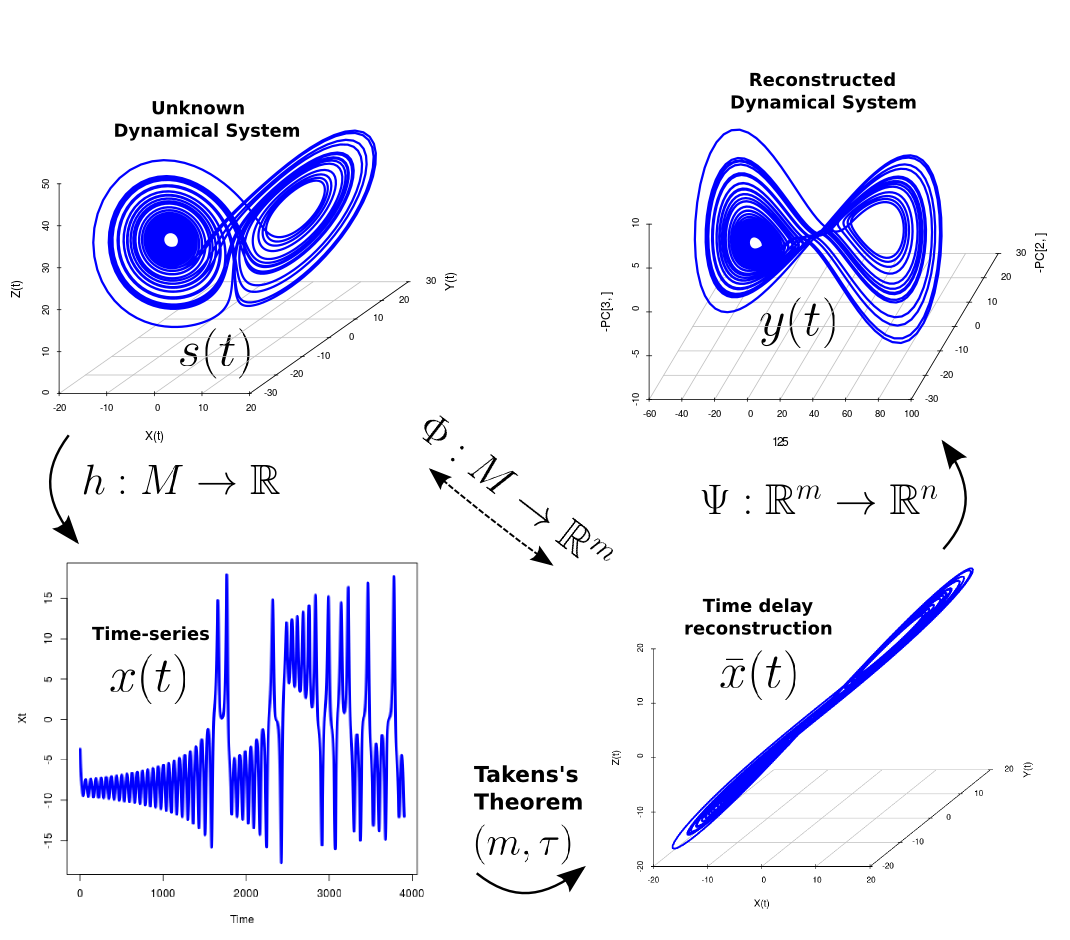
\includegraphics[width=0.43\textwidth]{takens_theorem_v6}
\caption[PA]{The reconstruction problem. The figure is based on the work of Uzal 
\textit{et al.} \cite{Uzal2011}.}
\label{fig:takens_theorem}
\end{figure}

\subsection{Embedding Parameters $m$ and $\tau$}
Given any time series $x(t)$, the time delay reconstruction 
system, $\overline{x}(t)$, is easy to implement. For this work, Cao's 
method \cite{Cao1997}, a modification of the False Nearest Neighbours 
(FNN) algorithm, and mutual information algorithm by 
Fraser \textit{et al.} \cite{Fraser1986} have been used to calculate minimum 
embedding parameters ($m_{min}$, $\tau_{min}$).


\subsubsection{Minimum Embedding Dimension}
Cao's method \cite{Cao1997} for computing the minimal embedding 
dimension is based on the mean values $E1(d)$ and $E2(d)$ 
where $d$ is a given embedding dimension value.

$E1(d)$ is used to obtain the minimal dimension $m_{min}$ 
and stops changing when the time series comes from an 
attractor (Figure~\ref{fig:e1e2} B). We computed $E1(d)$ values for 
$1 \leq \tau \leq 10$ to exemplify the minor dependency of $\tau$ 
given periodic, chaotic and random time series (Figures~\ref{fig:e1e2} (A,B,C)).

The second of these values, $E2(d)$, is used to distinguish 
deterministic signals from random signals in which case 
the $E2(d)$ values for random signals will be approximately equal to 1 for 
any $d$ (Figure~\ref{fig:e1e2} F).
Similarly, we computed $E2(d)$ values 
for periodic, chaotic and random time series, to exemplify 
the no significative dependency on $\tau$, where $1 \leq \tau \leq 10$ 
(Figures~\ref{fig:e1e2} (D,E,F)).

Cao's method is a modified version of the FNN method, 
and $E1(d)$ and $E2(d)$ values are only dependant on $m$ and 
$\tau$ \cite{Cao1997}.
\begin{figure}[!htb]
\centering    
 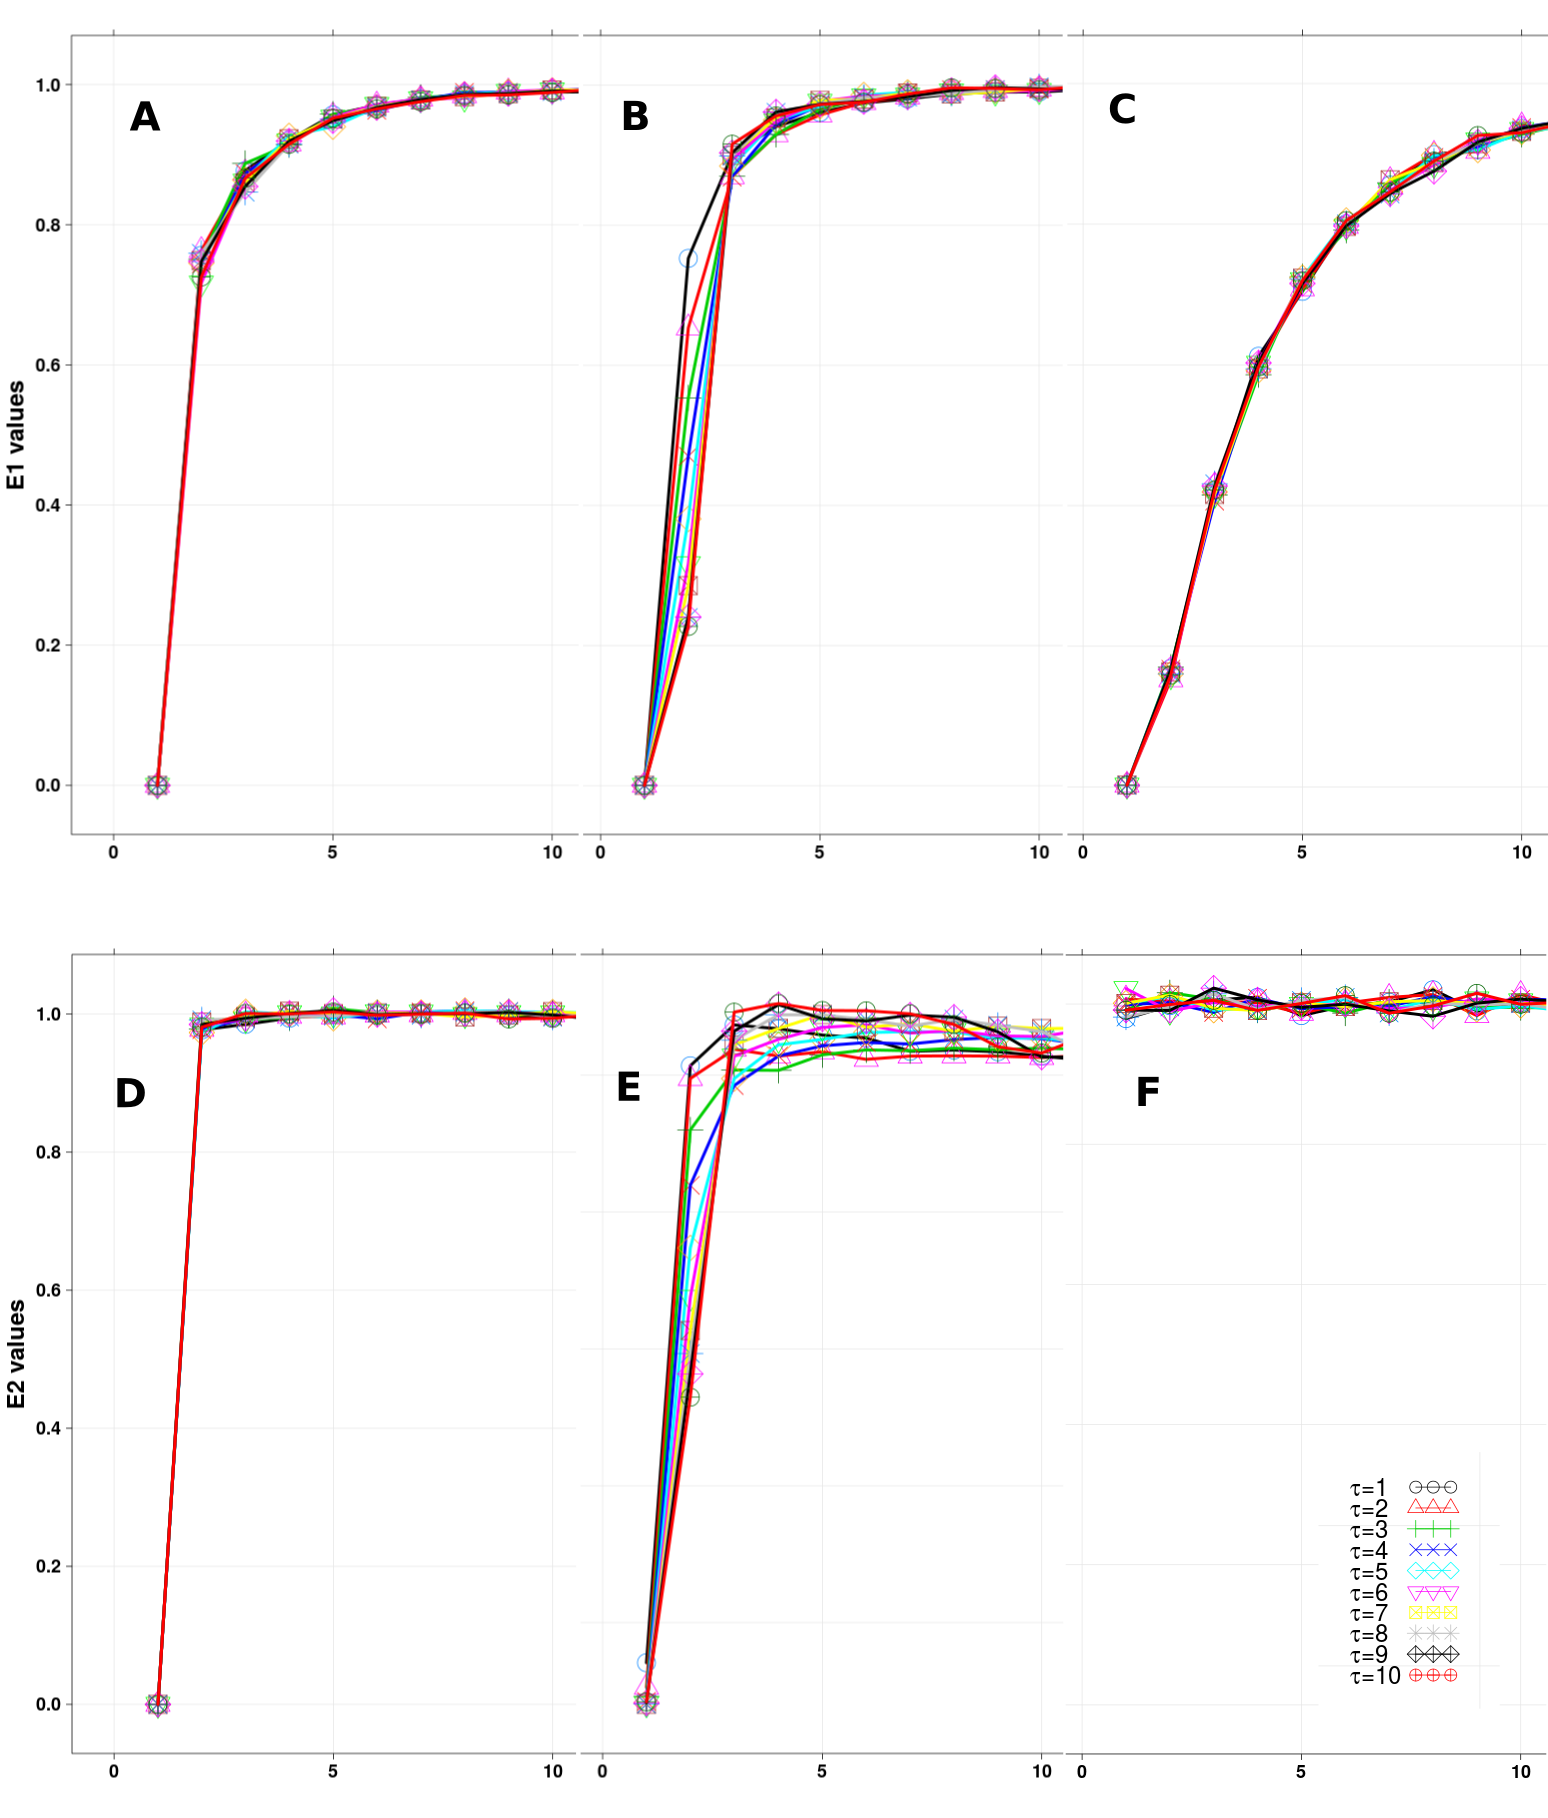
\includegraphics[width=0.45\textwidth]{e1e2_v00}
\caption[PA]{The values of $E1(d)$ and $E2(d)$ with different time-delay 
embedding parameters from periodic (A,D), chaotic (B,E) and random (C,F) 
time series.}
\label{fig:e1e2}
\end{figure}

\subsubsection{Minimum Time-delay Embedding}
The method of choosing the minimum time-delay embedding, 
$\tau_{min}$, was proposed by Fraser \textit{et al.} \cite{Fraser1986} in which 
the first minimum of the mutual information graph is chosen 
to estimate the minimal time-delay embedding parameter. For 
instance, Figure~\ref{fig:mi}  illustrates the mutual information from 
periodic, chaotic and random time series.
The local minimum for the Chaotic series in Figure~\ref{fig:mi} is $\tau_{min} = 18$.
On the other hand, for the random time series, the mutual information plot has
no local minimum and values are monotonically decreasing which means that $\tau_{min} = 1$
\cite{Fraser1986}. Further research has to be done when
data comes from a periodic time series since its minimum appears at  $\tau_{min} = 3$.

\begin{figure}[!htb]
\centering    
 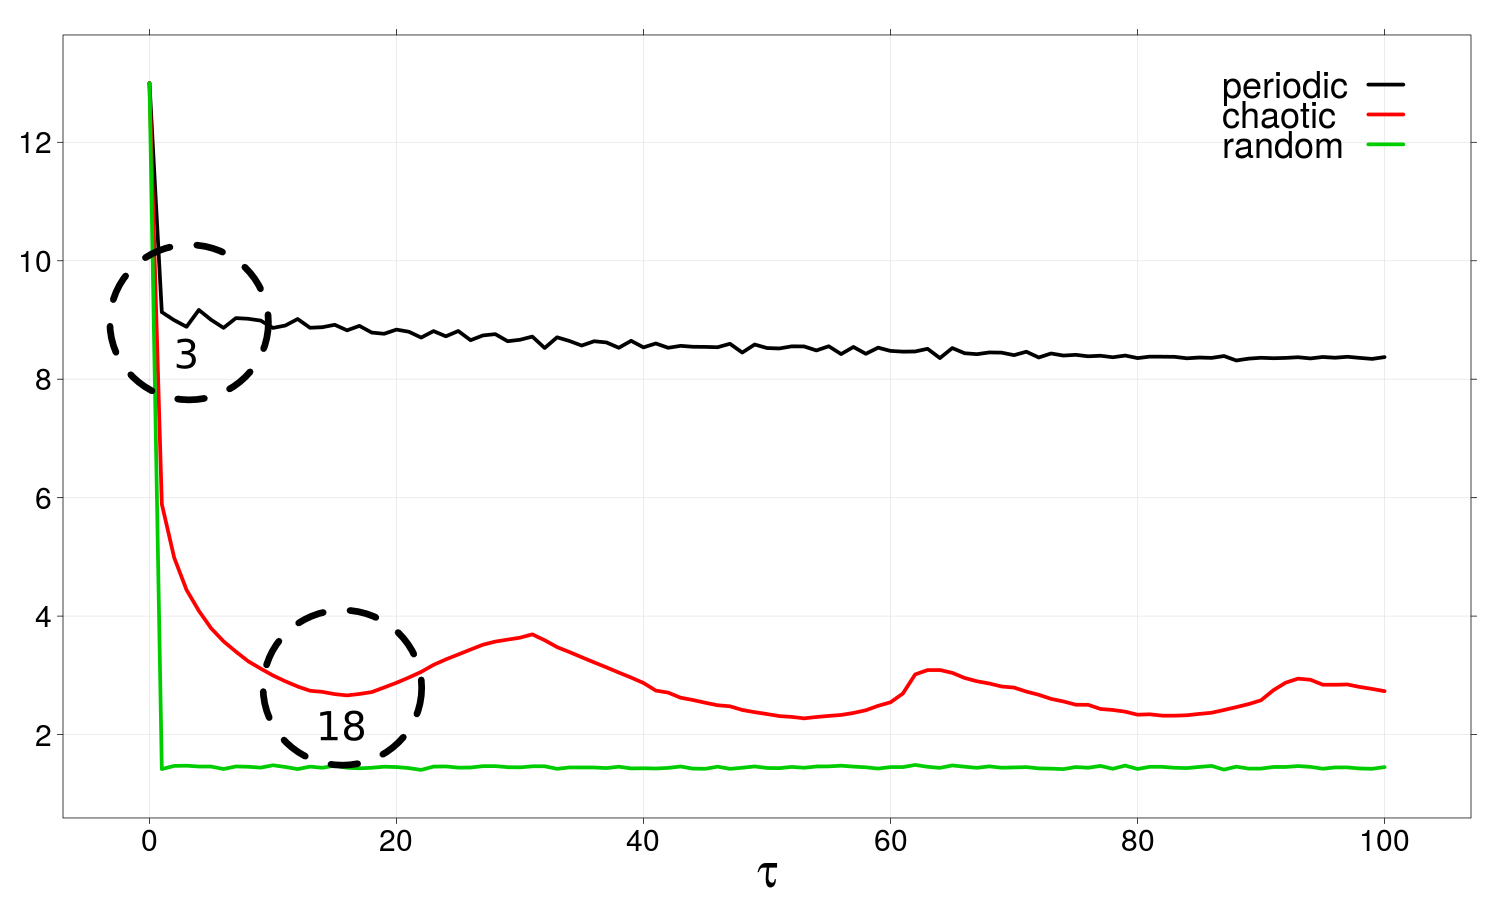
\includegraphics[width=0.45\textwidth]{mi_values_v02}
\caption[PA]{Mutual information plots from periodic, chaotic and random time series.}
\label{fig:mi}
\end{figure}

\subsubsection{Embedding Parameters Setbacks}
Although the time-delay embedding method using inertial 
sensors has been used in gait recognition \cite{Sama2013}, gait stability 
\cite{Gouwanda2012} and walking, running and cycling activities \cite{Frank2010},
some problems with the minimal embedding parameter estimation  
($m_{min}$ and $\tau_{min}$) still remain to be solved.

Sama \textit{et al.} \cite{Sama2013} and Gouwanda \textit{et al.} \cite{Gouwanda2012} estimated 
the minimal embedded dimension ($m_{min}$) with the False Nearest 
Neighbours (FNN) method. However, Cao \cite{Cao1997} pointed 
out that the FNN algorithm introduces new parameters 
($R_{tol}$ and $A_{tol}$) that lead to different results and cannot 
differentiate random series from deterministic series. Frank 
\textit{et al.} \cite{Frank2010} proposed a grid search method to find the minimal 
embedded parameters, but there are no details about their 
approach.

In the case of the minimal time delay embedding value, 
$\tau_{min}$, Fojt \textit{et al.} \cite{Fojt1998} mentioned a method in which the 
chosen $\tau$ is made in function of filling the space of the 
reconstructed system; however, Fojt \textit{et al.} \cite{Fojt1998} mentioned that 
``it is a rough estimation based on a graphical procedure.''
Although, Sama \textit{et al.} \cite{Sama2013} computed $\tau_{min}$ using the method 
proposed by Fraser \textit{et al.} \cite{Fraser1986}, they pointed that the chosen 
$\tau_{min}$ largely depend on the application.



\section{The Activity Recognition Chain}
\begin{figure*}
\centering    
 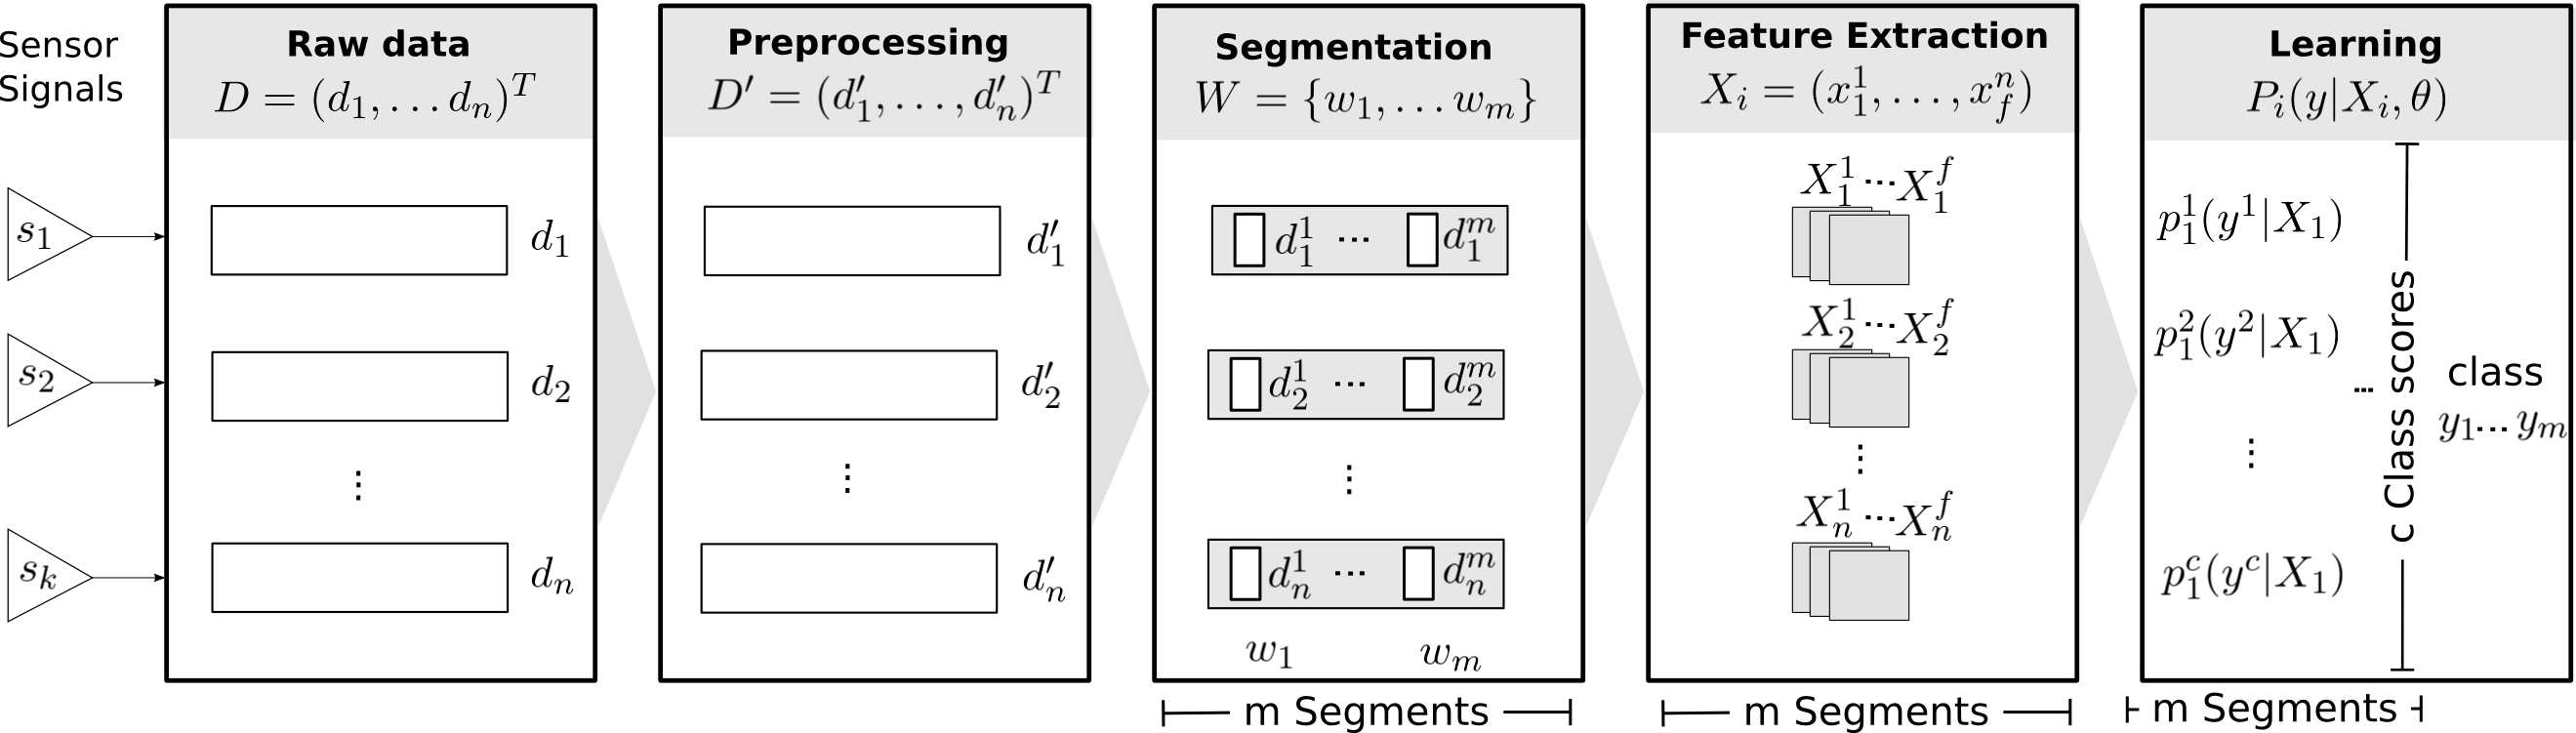
\includegraphics[width=\textwidth]{ARC02}
\caption[PA]{Typical activity recognition chain (ARC) to identify activities or gestures
from body-worn inertial sensors. 
Diagram is replicated from the work of Bulling \textit{et al.} \cite{bulling2014}.}
\label{fig:arc}
\end{figure*}
Bulling \textit{et al.} \cite{bulling2014} reviewed the state of the art of HAR using 
body-worn inertial sensors. Figure~\ref{fig:arc} illustrates the typical 
activity recognition chain (ARC) to identify activities with 
body-worn sensors.

The first stage of the ARC is the raw data collection 
from several sensors attached to different parts of the body. 
Data from sensors over a given time, $s_i$, provide multiple time series $d_n$, 
(e.g. $d_1, d_2, d_3$ for 3-D acceleration referred to as x, y and z direction)
\begin{equation}
s_i = (d_1, d_2,\dots,d_n), \quad \mbox{for } i=1, \dots,k
\end{equation} 
where $k$ denotes the number of sensors and $n$ the number 
of degrees of freedom of the inertial sensor.

In the preprocessing stage of the ARC, raw multivariable time series 
are transformed into a pre-processed time series 
$D'= (d'_1, \dots, d'_n )^T$, where $d'_i$ is one dimension of the data 
for the preprocessed time series and $n$ is the number of total 
data dimensions. Different methods for the preprocessing 
tasks may be applied to the raw data (e.g. synchronisation, 
calibration, unit conversion, normalisation, resampling, 
denoising  or baseline drift removal \cite{bulling2014}).

The stage of data segmentation identifies segments 
within the continuous data stream that are likely to have 
information about activities. The segmentation stage creates 
a set of segments $w_m$ such that 
\begin{equation}
W = \{   w_1, \dots, w_m  \},
\end{equation} 
where $m$ corresponds to the number of segments. Since the 
segmentation of the data is a difficult problem, there are 
various methods in the literature to solve this problem: sliding 
window, energy-based segmentation, rest-position segmentation, 
additional sensors and external context sources.


In the feature extraction stage, a feature extraction function 
$F$ reduces the signals $D'$  into segmented signals $W$.
The total number of features $X_i$ is the feature space.
\begin{equation}
X_i = F ( D', w_i)
\end{equation} 
In the literature on activity recognition, different methods 
for feature extraction can be found including signal-based 
features, body model features, event-based features, 
multilevel features or automatic feature ranking and selection.


Machine learning tools have been used in HAR over 
the last 15 years so as to describe, analyse and predict human 
activities \cite{bulling2014}. However, the chosen approach is subject to 
computational complexity, recognition performance or latency.
Generally for the learning stage, a training data set 
$T = \{ X_i, y_i \}  ^N _ {i=1}$ is computed prior to the classification 
with $N$ pairs of feature vectors $X_i$ and ground truth labels 
$y^i$ (possible activities to recognise). For this stage, model 
parameters $\theta$ can be learned to decrease the classification 
error on $T$. Then, with the trained model $T$, each feature 
vector $X_i$  is mapped to a set of class labels $Y= \{ y^1, \dots , y^c \}$ 
with scores $P_i = \{ p^1_i, \dots, p^c_i \}$:
\begin{equation}
p_i ( y \mid X_i, \theta) = I (X_i, \theta), \quad \mbox{ for } y \in Y
\end{equation} 
and inference method $I$. Finally, the classification output $y_i$ 
is computed with the maximum score $P_i$
\begin{equation}
y_i  = 
\underset{ y \in Y, p \in P_i }{\text{argmax}}   p(y | X_i, \theta)
\end{equation} 
The most common classification algorithms are: decision 
trees, Bayesian models, domain transform, fuzzy logic, 
Markov models, support vector machines (SVM), artificial 
neural networks (ANN) and ensembles of classifiers \cite{Lara2013}.


Similarly, when the recognition of activities can miss,
confuse or falsely recognise activities that did occur, several 
metrics can be used to optimise the classification. Some 
of the metrics are confusion matrices, accuracy, precision, 
recall, and F-scores, decision-independent Precision-Recall 
or receiver operating characteristic curves (ROC curves) \cite{bulling2014}.

The state-of-the-art on ARC framework is far from 
quantifying the repeatability and consistency of human activities.
The reasons for this are: i) ARC frameworks have only been
applied to identify the activities; and ii) once the activities
have been identified, further analysis has to be done to
learn the variability of the activities. The quantification of 
the skillfulness in terms of the variability and consistency 
of the human activities is an example. However, little work
has been done in this area. 
Tessendorf \textit{et al.} \cite{Tessendorf2011}, for instance,
proposed an ARC framework in which only the raw data 
collection and indicators of the rowing technique are used 
to quantify the rowing techniques of ambitious amateurs 
and world-class rowers. Velloso \textit{et al.} \cite{Velloso2013a,Velloso2013b} presented
a framework that is more related to the ARC; this framework
includes data collection (angle joints from kinect sensor),
preprocessing (converting the joints' position coordinates),
segmentation (specific intervals of time or every repetition of
the activity), feature extraction (performing statistical analysis
when the event is triggered) and classification (threshold
operations).



\section{Artificial Signals}
To understand the possible sources of variability in dance activities, I
followed the method of Hammerla \textit{et al.} \cite{hammerla2011} which can be
useful to model: i) noise in sensors, ii) properties of activities and iii)
properties of people.

The proposal of Hammerla \emph{et al.} \cite{hammerla2011}
is aimed to examine the effects of
variability in the precision of motion  (additive noise) 
and in the strategy of motion  (structural noise) of 
activities using artificial signals.

Additive noise is normalised noise with variance $\sigma_a ^2$ added to the
sinusoid signal $S$: 
\begin{equation}
 S^a = S + \textbf{N}(0, \sigma_a ^2)
\end{equation} 

Structural noise is a sinusoid signal distorted with different variance 
in frequency and amplitude $\sigma_s ^2$ and window length $w_s$. 
Algorithm 1 describes the creation of structural noise.
To make the data less redundant for possible variations of environmental 
conditions or body-worn sensor mobility in users, the data is whitened 
(i.e. data is normalised to have zero mean and unit variance) 


% http://tex.stackexchange.com/questions/219816/algorithm-in-ieee-format
\begin{algorithm}[H]
\caption{Structural Noise}
\begin{algorithmic}[1]
 \renewcommand{\algorithmicrequire}{\textbf{Input:}}
 \renewcommand{\algorithmicensure}{\textbf{Output:}}
 \REQUIRE time-series $S^a$, variance $\sigma_s ^2$, window length $w_s$
 \ENSURE  Structurally distorted signal $S^s$
  \FOR {$j = 1$ to $L$, $j=j+w_s$}
  \STATE $\textbf{u'} \leftarrow \textbf{N}(0, \sigma_s ^2)$
  \STATE $S^{a} =$ sinusoid with frequency $| \textbf{u'} |$ and variance $\sigma_a ^2$ of length $w_s$
  \STATE $S^s_{j \rightarrow j+w_s}  = S^s_{j \rightarrow j+w_s}  + S^{a} \times   \sigma_s ^2 $
  \ENDFOR
  \\ $S^s= whiten (S^s)$
 \RETURN $S^s$
\end{algorithmic}
\end{algorithm}


By varying both $\sigma_a ^2$ and $\sigma_s ^2$ is possible to simulate and
control the additive noise and the structural noise in the structure of the
human activity. For example, low values of $\sigma_a ^2$ are associated with
precise movements while low values of $\sigma_s ^2$ correspond to a well chosen
strategy for a movement (Figure~\ref{fig:sn}).

\begin{figure}[!htb]
\centering 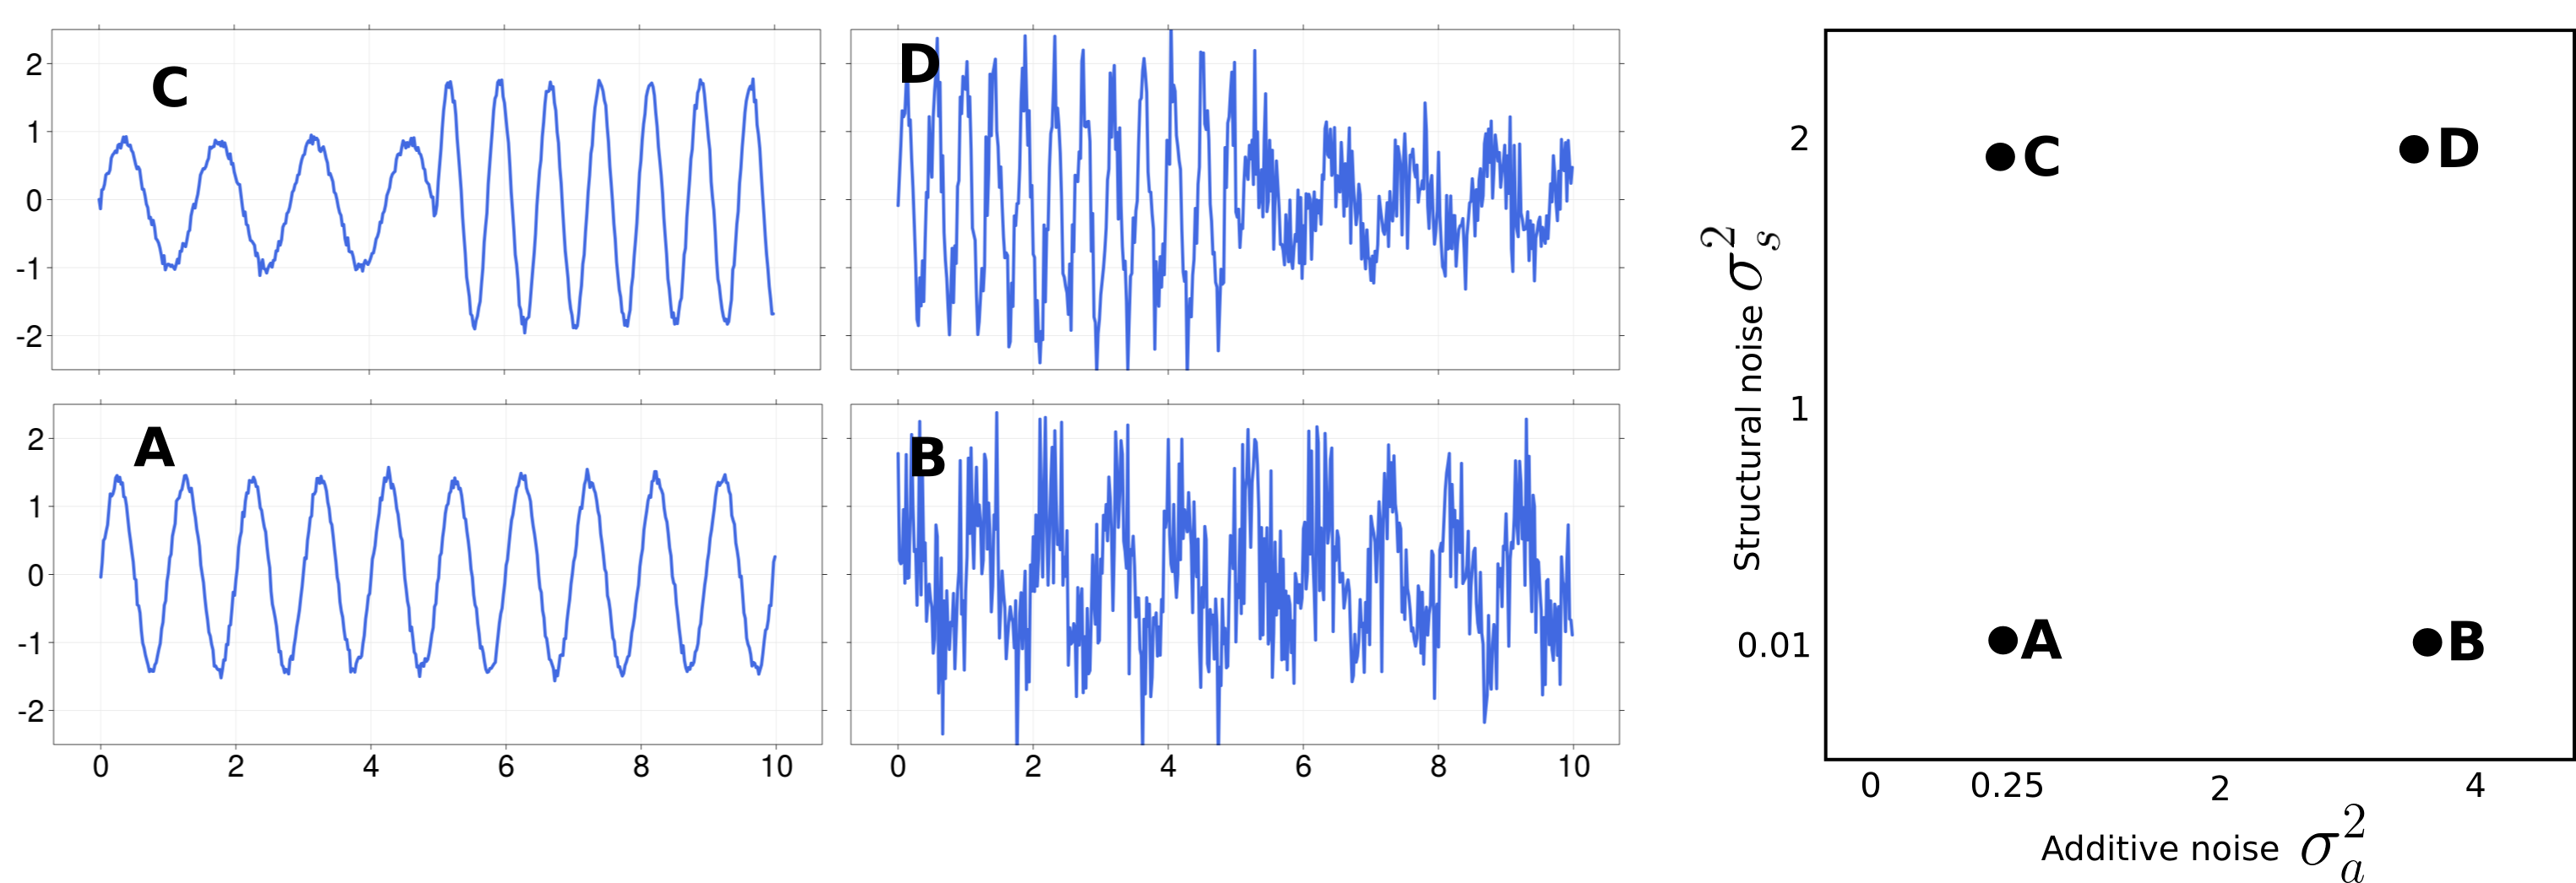
\includegraphics[width=0.45\textwidth]{impactofnoise01}
\caption[PA]{Graphs (A, B, C and D) present the variability of additive noise
  ($\sigma_a ^2$) and structural noise ($\sigma_s ^2$ ) on the sinusoid signals
  with $w_s=500$ according to the parameters indicated on the left plot.}
\label{fig:sn}
\end{figure}

For graphs in Figure~\ref{fig:sn}, the base frequency of the sinusoidal is 1 Hz
sampled at 50Hz with an amplitude 1 and window length of 250 samples.


\section{Data Collection and Analysis}

\subsection{Data Collection}
Data from 3-axis accelerometer, gyroscope and magnetometer 
were collected at a sampling rate of 50 Hz using four Razor 
9DOF IMUs with Bluetooth (Adeunis ARF7044). The IMUs were 
attached to custom-made bracelets worn by participants: 
two sensors were located in the front part of the right 
and left ankle, one in the back of the hip and 
another in back of the neck.


\subsection{Participants}
Thirteen participants with different years of experience in
dancing salsa were invited, one (male) expert dancer
(14 years of experience), one intermediate (male) dancer
(4 years of experience) and eleven non-dancers. The
non-dancers were students of engineering (mean age 22 years; 4
female, 7 male). While 2 of these dancers (1 male and 
1 female) had danced previously, none of this group has
experience in Salsa dancing. For this report, we focus on the 
data from 3 individual dancers an expert, intermediate and
non-dancer, respectively.
\begin{figure}[!htb]
\centering    
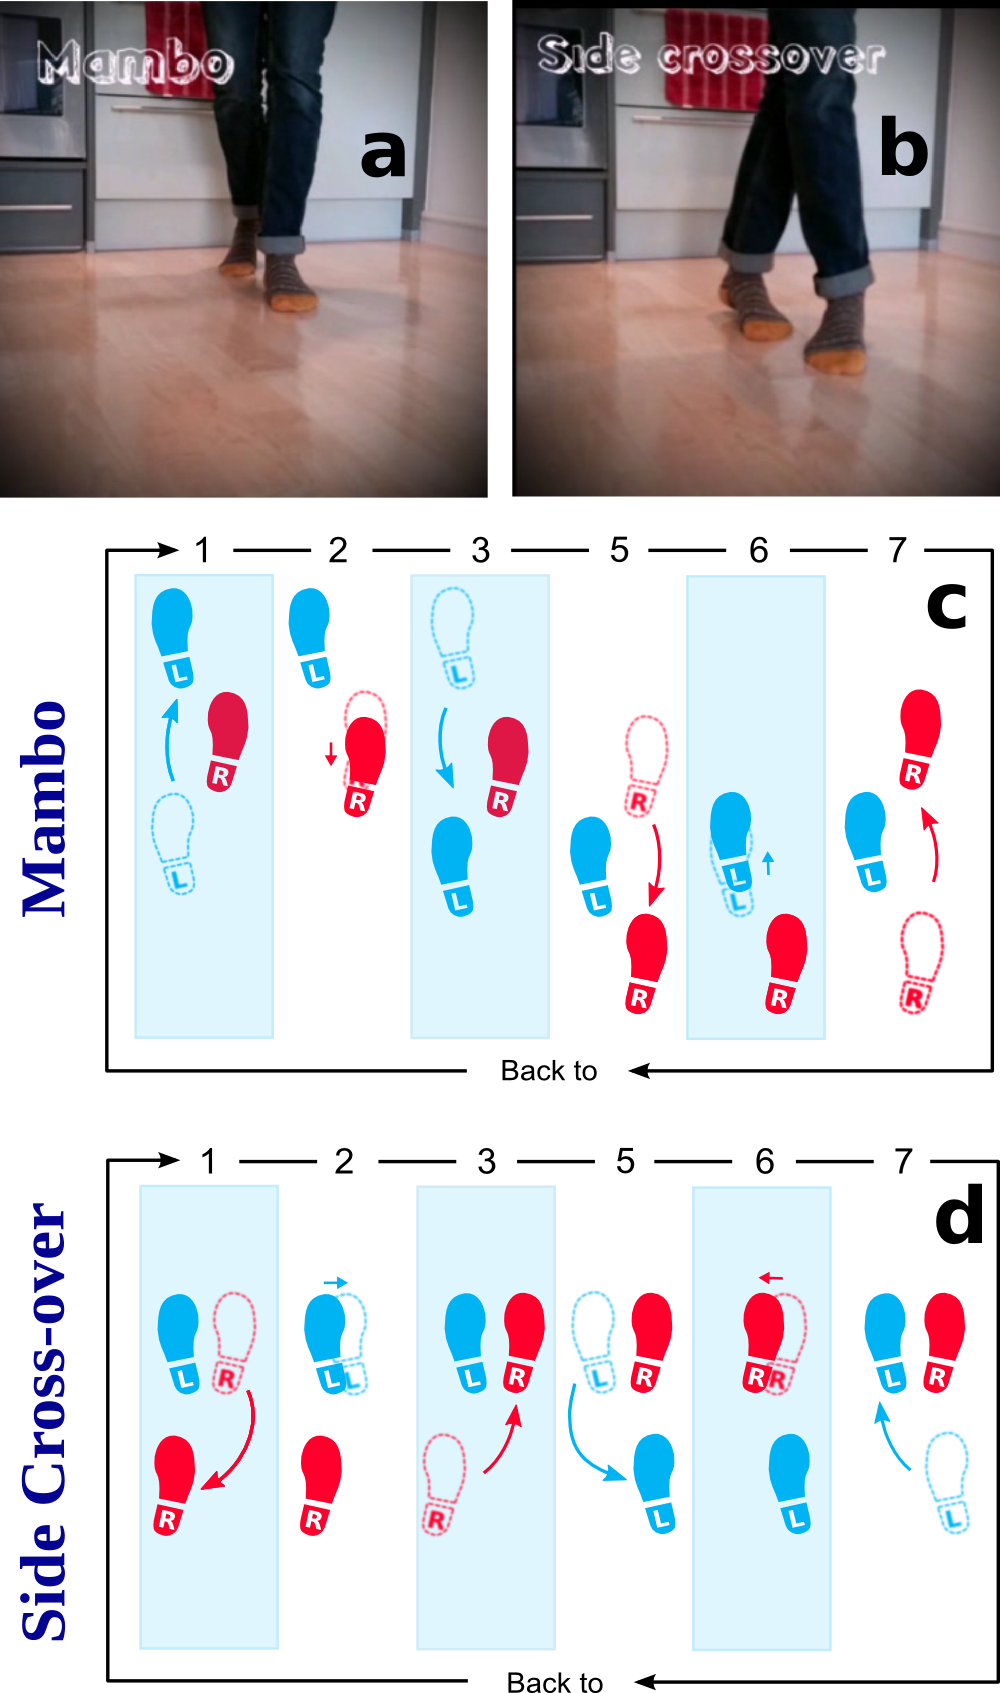
\includegraphics[width=0.45\textwidth]{steps_v00}
\caption[PA]{Salsa step patterns: (a) mambo (step 1) and (b) side crossover
(step 2). Foot patterns for (c) the mambo style (step 1) and (d) the side crossover style (step 2).}
\label{fig:steps}
\end{figure}




\subsection{Experimental Conditions}
The design of the experiment met the University of Birmingham
ethics approval and all participants provided informed consent 
prior to participation. On arrival, participants were assisted 
in attaching the IMUs and the manner in which data were collected 
from these IMUs was demonstrated to them. 
Once they were comfortable with the fit of IMUs, the experimental 
task was explained to them.

Each participant was shown a series of video clips (recorded
by the expert dancer) demonstrating Salsa steps. Each video
clip showed one step repeated several times for 20 seconds.
For the analysis in this paper, we report two Salsa step patterns: 
step 1 = mambo and step 2 = side crossover (Figure~\ref{fig:steps}).
Participants watched the video clip and were then asked to
copy the steps in time to music. The video was played during
the data collection (so that participants did not have to rely on
their memory of the steps).

Data were collected from the IMUs and recorded. 
For this report, the analysis reported will focus on data taken from the
sensor mounted on the left ankle.


\subsection{Framework for the Experiment}
The raw data is collected from 
accelerometer ($a_{ \{ x,y,z \} }$), gyroscope ($g_{ \{ x,y,z \} }$) 
and magnetometer($m_{ \{ x,y,z \} }$) sensors. 
Then, the time-series $a_x$ with a length of $N$ samples is used to obtain 
the time-delay embedded matrix, $\boldsymbol{E} a_{x}$, with $m$ rows and $N-(m-1)\tau$ columns. 
Finally, the PCA algorithm is applied so as to obtain via eigenvalues 
($\lambda_1,\ldots,\lambda_m$), eigenvectors ($v_1,\ldots,v_m$) and the principal components 
($PC_1,\ldots,PC_m$) of the time-delay embedded phase space (Figure \ref{fig:raw_takens_pca}).
\begin{figure}[!htb]
\centering
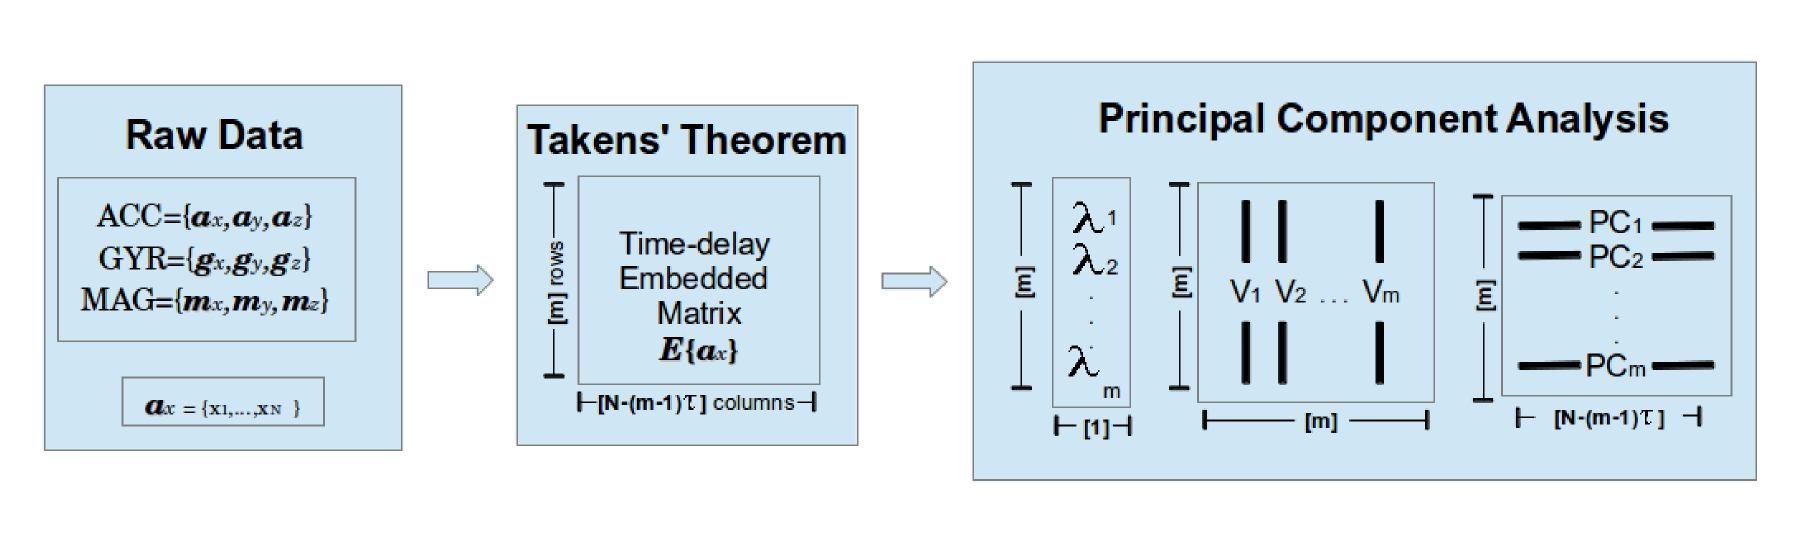
\includegraphics[width=0.45\textwidth]{diagram_v10}
\caption[PA]{Diagram for the phase space reconstruction.}
\label{fig:raw_takens_pca}
\end{figure}


\subsection{Estimation of the Minimal time-delay Embedding Parameters}
Data from the inertial sensor for the left ankle of the expert 
dancer were used to compute $E1(d)$ and $E2(d)$. These 
values are computed using a time-series, for instance, $m_x$
so as to obtain four curves that correspond to each delay 
embedding parameters ($\tau=1,2,3,4$) for dimension that 
are in the range $0 \leq d \leq 40$. From $E1(d)$ values (Figures~\ref{fig:e1e2exp}) 
one can notice that the minimal value for the embedded 
dimension is approximately equal to $m_{min} \approx 10$. Generally, 
the $E2(d)$ values show that data from $m_x$ and $m_y$ 
are more noisier than that from $m_z$; however, $E2(d)$ values 
from step 2 are less noisier than that from step 1  (Figures~\ref{fig:e1e2exp}).
\begin{figure}[!htb]
\centering    
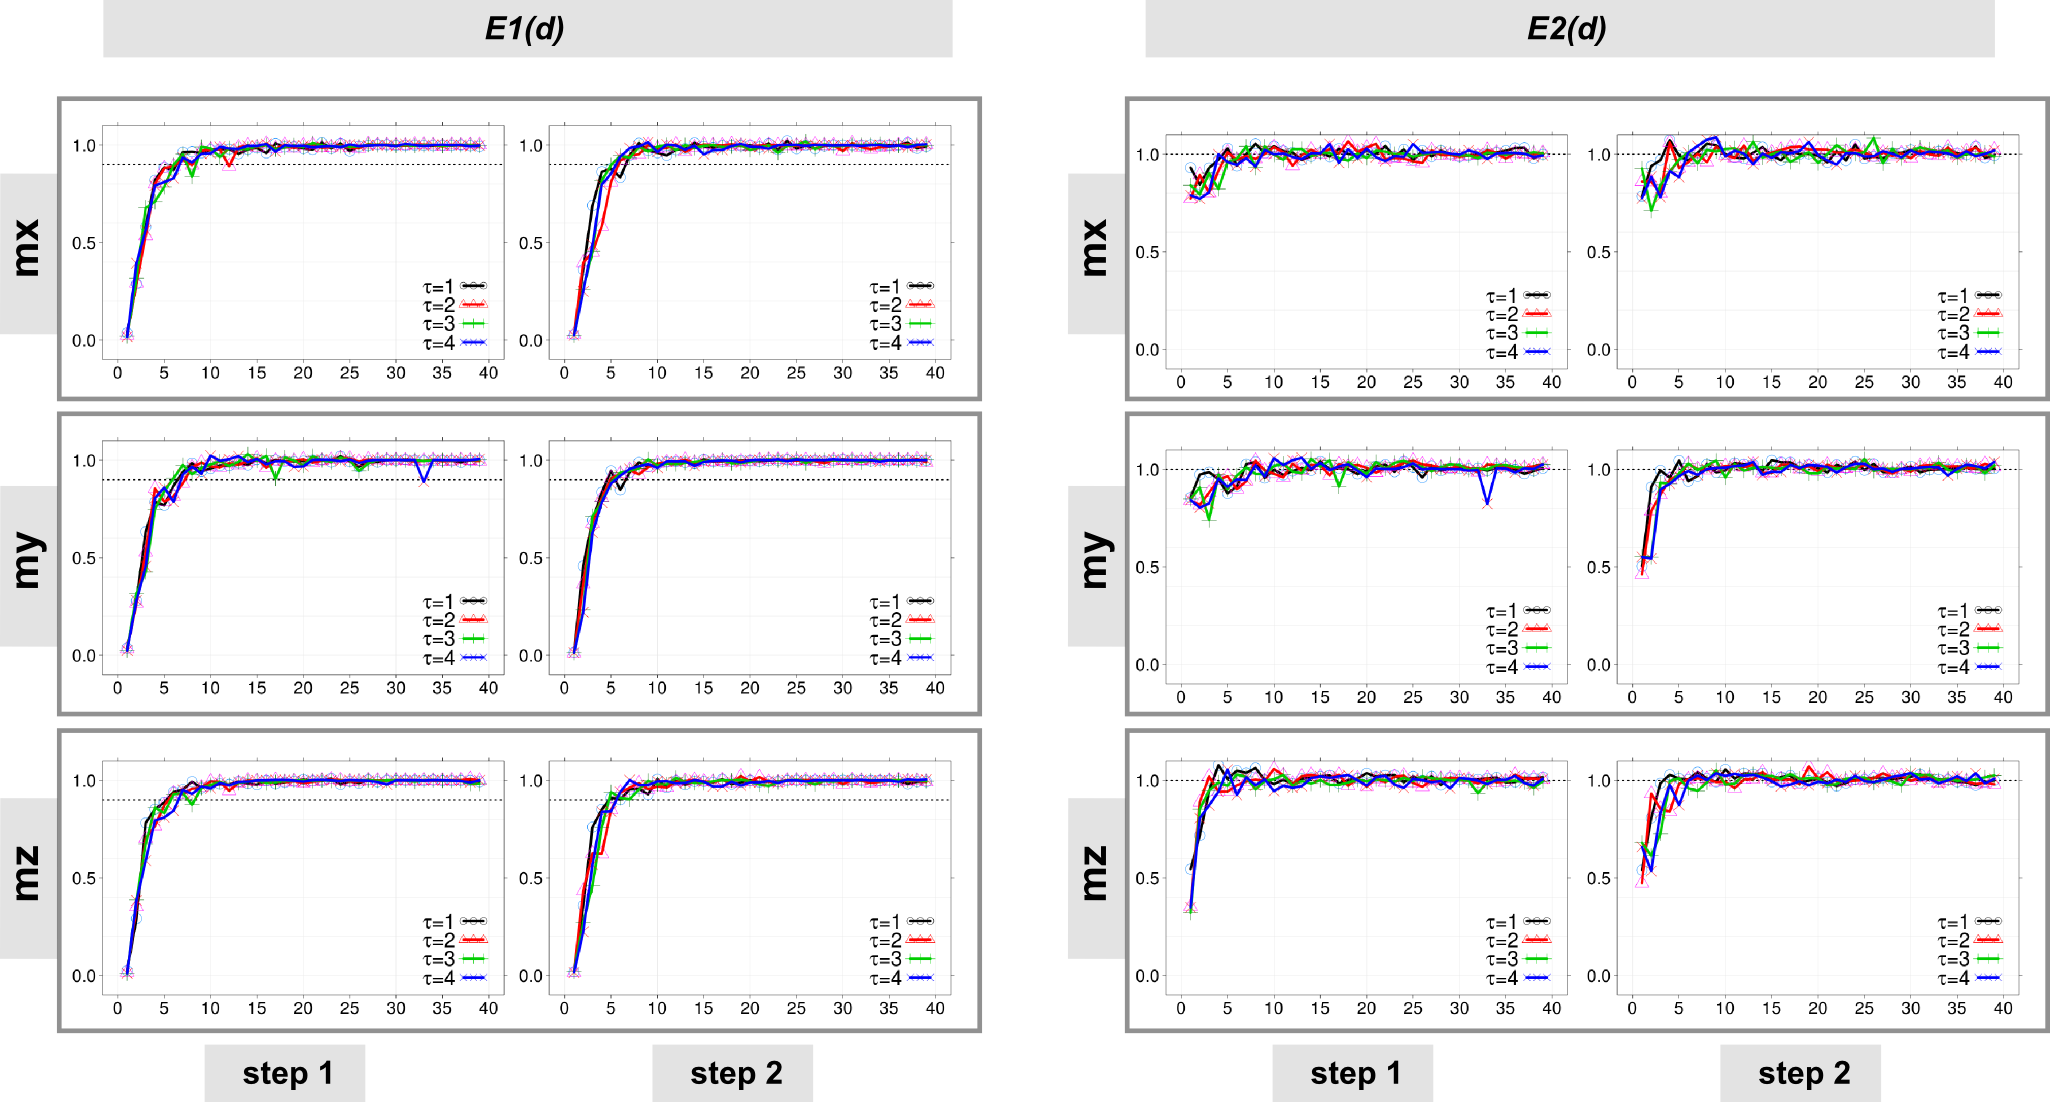
\includegraphics[width=0.45\textwidth]{e1e2_values_expert}
\caption[PA]{$E1(d)$ and $E2(d)$ values for $\tau=1,2,3,4$ with $0 \leq d \leq 40$
from magnetometer sensor ($m_{ \{ x,y,z \} }$) of the expert dancer for two dance steps.
The dashed straight line for $E1(d)$ and $E1(d)$ corresponds to the value 0.9 and 1, respectively.}
\label{fig:e1e2exp}
\end{figure}
Independently of the sensors' axis or dance steps, different $\tau$ 
values provide approximately the same minimal embedding 
dimension ($m=10$) in $E1(d)$ values (Figures~\ref{fig:e1e2exp}). For the 
minimum time-delay embedding parameter, the mutual 
information plot is computed using the magnetometer sensor 
data $m_{ \{ x,y,z \} }$. The first minimum of the time-delay embedding 
for both plots using $m_z$ is at $\tau=6$ (Figure~\ref{fig:miplots}).
\begin{figure}[!htb]
\centering    
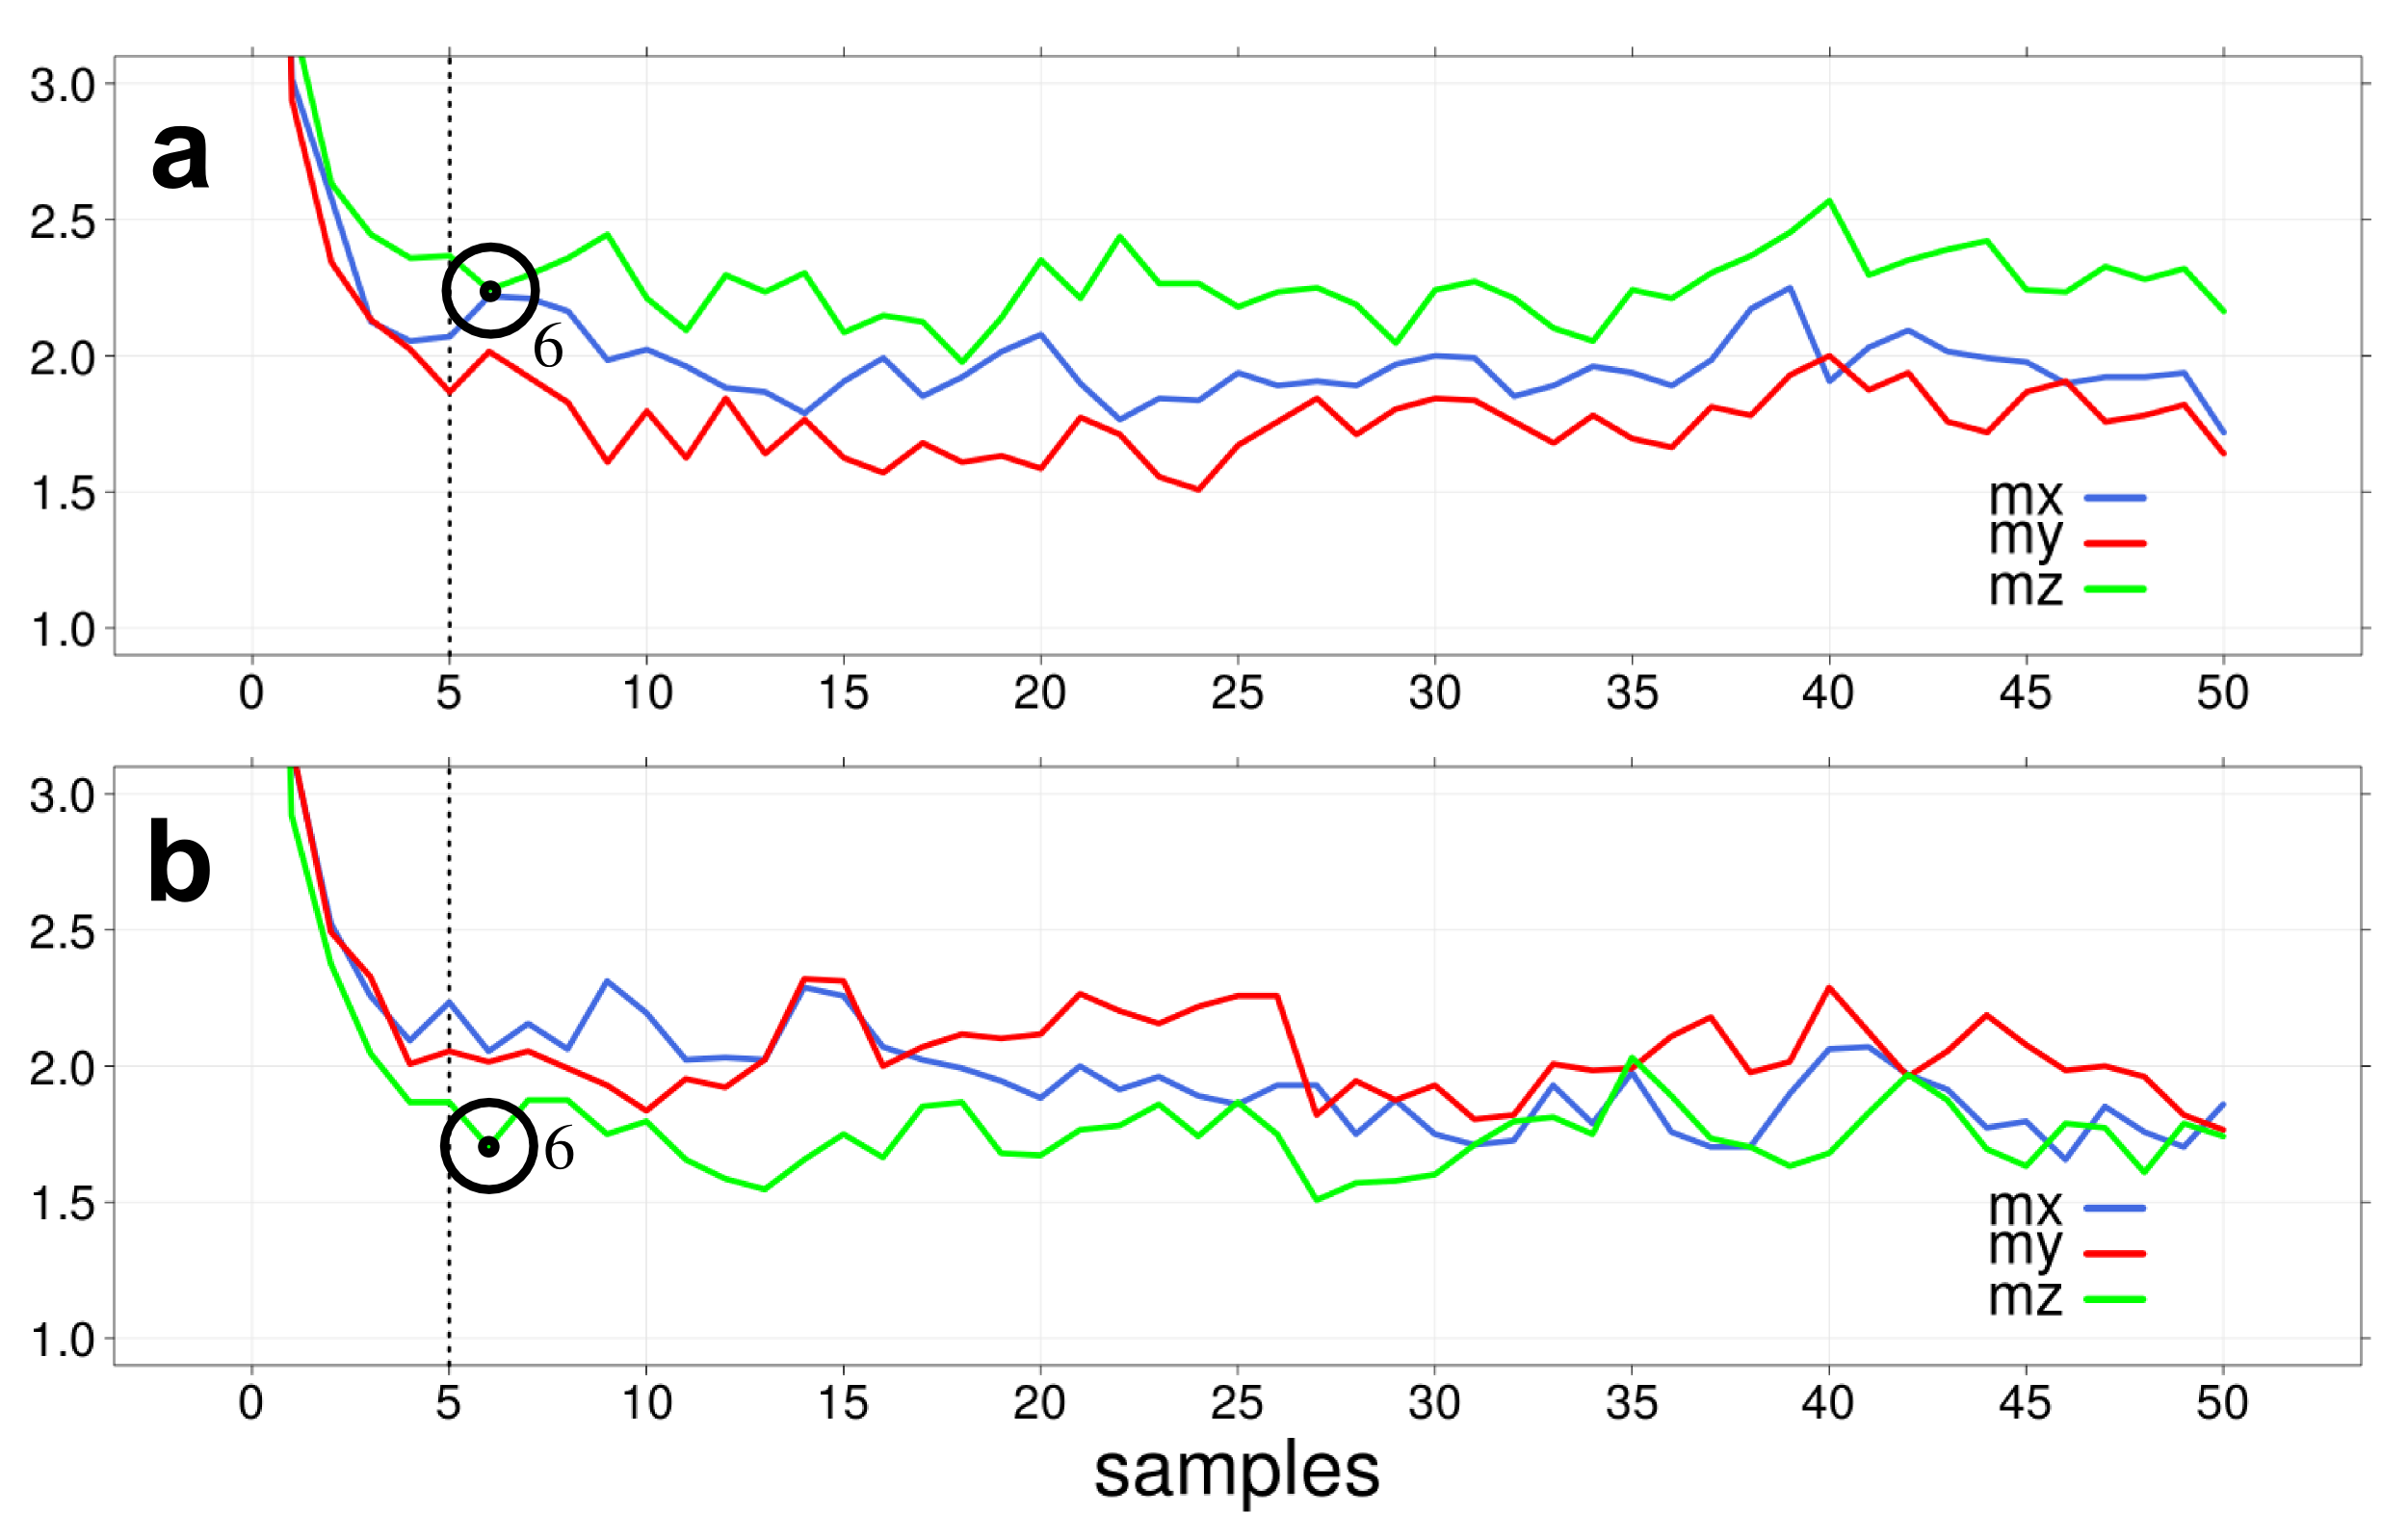
\includegraphics[width=0.45\textwidth]{miplots01}
\caption[PA]{
Mutual information values for $0 \leq \tau \leq 50$ from magnetometer sensor 
($m_{ \{ x,y,z \} }$) of the expert dancer for (a) step 1 and (b) step 2.
The vertical dashed straight line in both plots correspond to the value $\tau=5$.
The first minimum for both plots from $m_z$ is at $\tau=6$.}
\label{fig:miplots}
\end{figure}
We therefore computed time-delay 
embedded matrix with $m=10$ and $\tau = 6$ for each 
axis from the magnetometer sensors depicted in Figure \ref{fig:raw_takens_pca}.



\subsection{2-D Reconstructed State Spaces}

Figure~\ref{fig:skills} illustrates the 2-D reconstructed state space for the 
non-dancer, intermediate and expert dancers which visually 
helps us to distinguish different levels of dexterity. It is 
immediately noticeable that the shape of the state space 
for each level (novice, intermediate, expert) appear visually 
similar across step 1. As the participants are meant to be 
performing the same action, this similarity is to be expected.
However, the state spaces also show a tighter and less varied 
pattern for the expert than for the other dexterity levels. This 
suggests that the expert is producing more repeatable, more 
consistent actions than the other dexterity levels. While this 
is to be expected, the reconstructed state spaces provide 
interesting illustrations of this phenomenon.  For step 2, 
which is a more complicated sequence of movements, one 
can see a marked contrast across dexterity levels. Again, the 
expert is showing a consistent and repeatable action. The 
intermediate participant is showing a consistent action but 
this is different to that of the expert, and the novice is showing 
a pattern which appears disjointed and noisy. Indeed, 
for the novice dancer, the state space reconstruction of step 2 
seems to have more in common with their state space for 
step 1 than it does with the other dancers performing step 2.  
\begin{figure}[!htb]
  \centering
  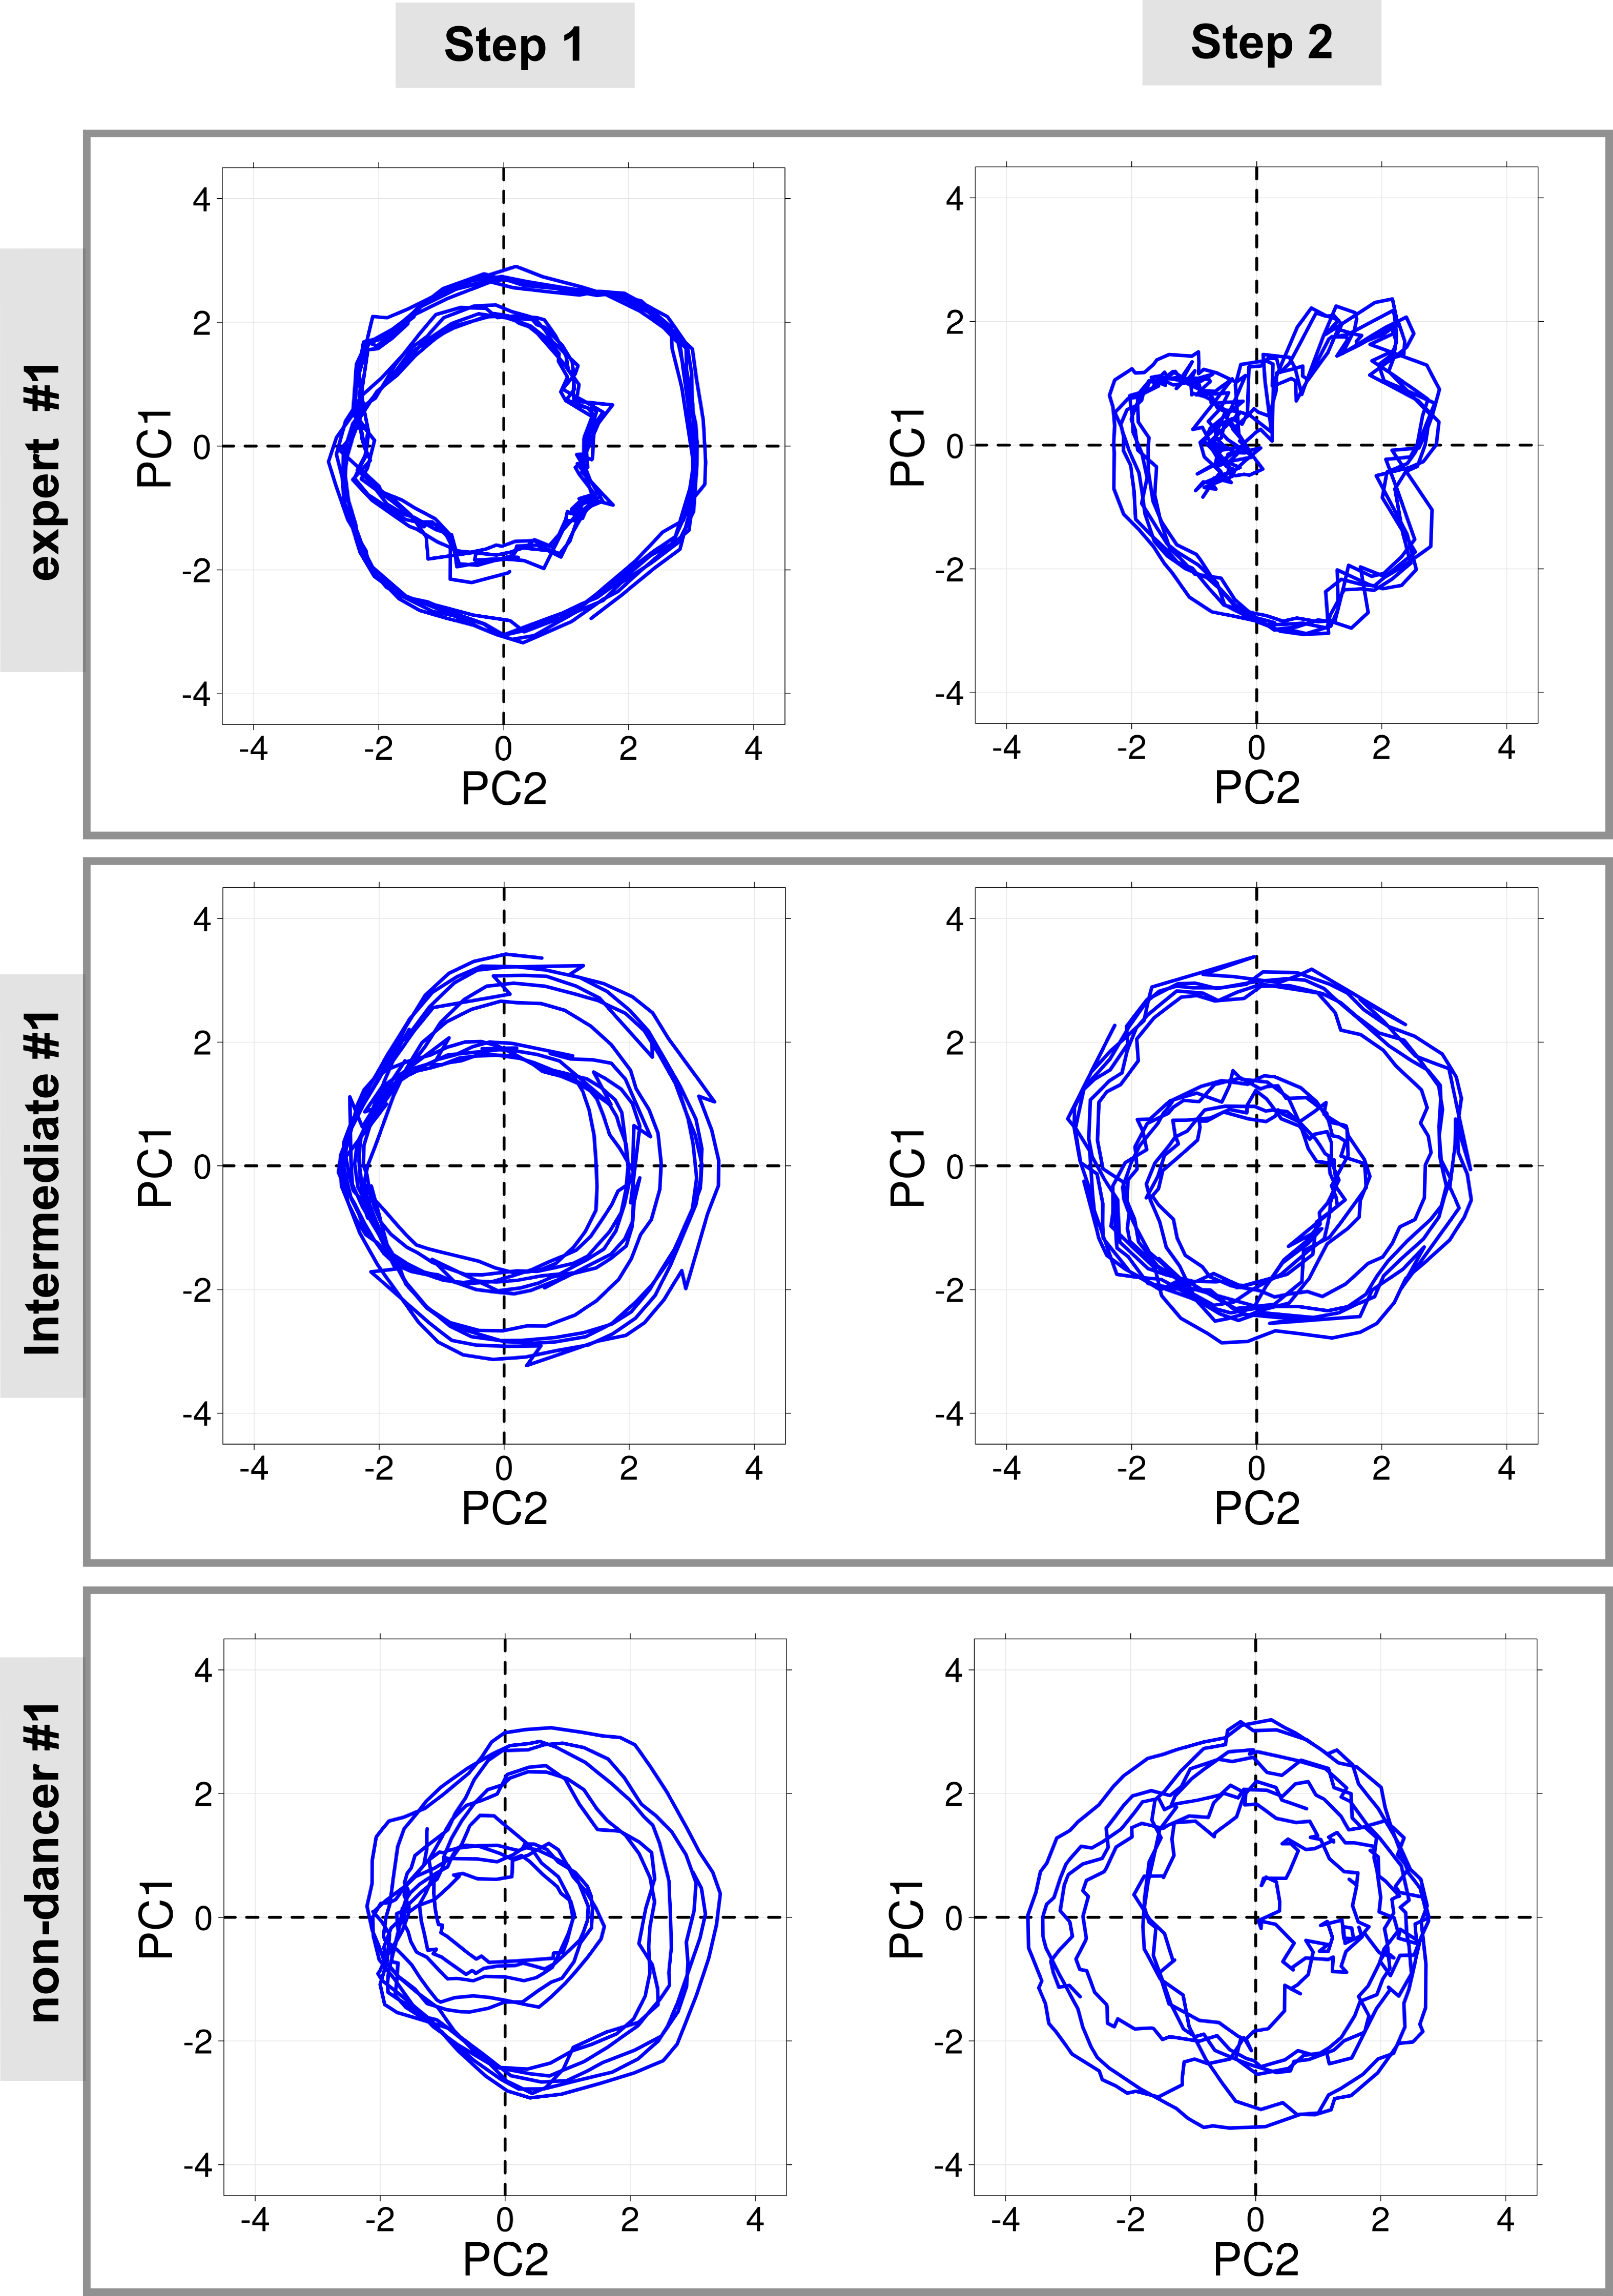
\includegraphics[width=0.45\textwidth]{rss00}
  \caption[PA]{2-D reconstructed state spaces for the expert, intermediate and
  non-dancer participants for step 1 ($m_z$ data) and step 2 ($m_y$ data).
  First two component of the PCA with embedding parameters ($m = 10$ and $\tau = 6$).}
  \label{fig:skills}
\end{figure}

Sama \textit{et al.} \cite{Sama2013} pointed out that the chosen $\tau_{min}$ largely 
depends on the application. In this case, the mutual information 
method indicates that $t_{min} =  6$; however, different 
values of $m$ and $\tau$ give different reconstructed state spaces 
(Figure ~\ref{fig:takens_problem}).



\begin{figure}[htbp!] 
\centering    
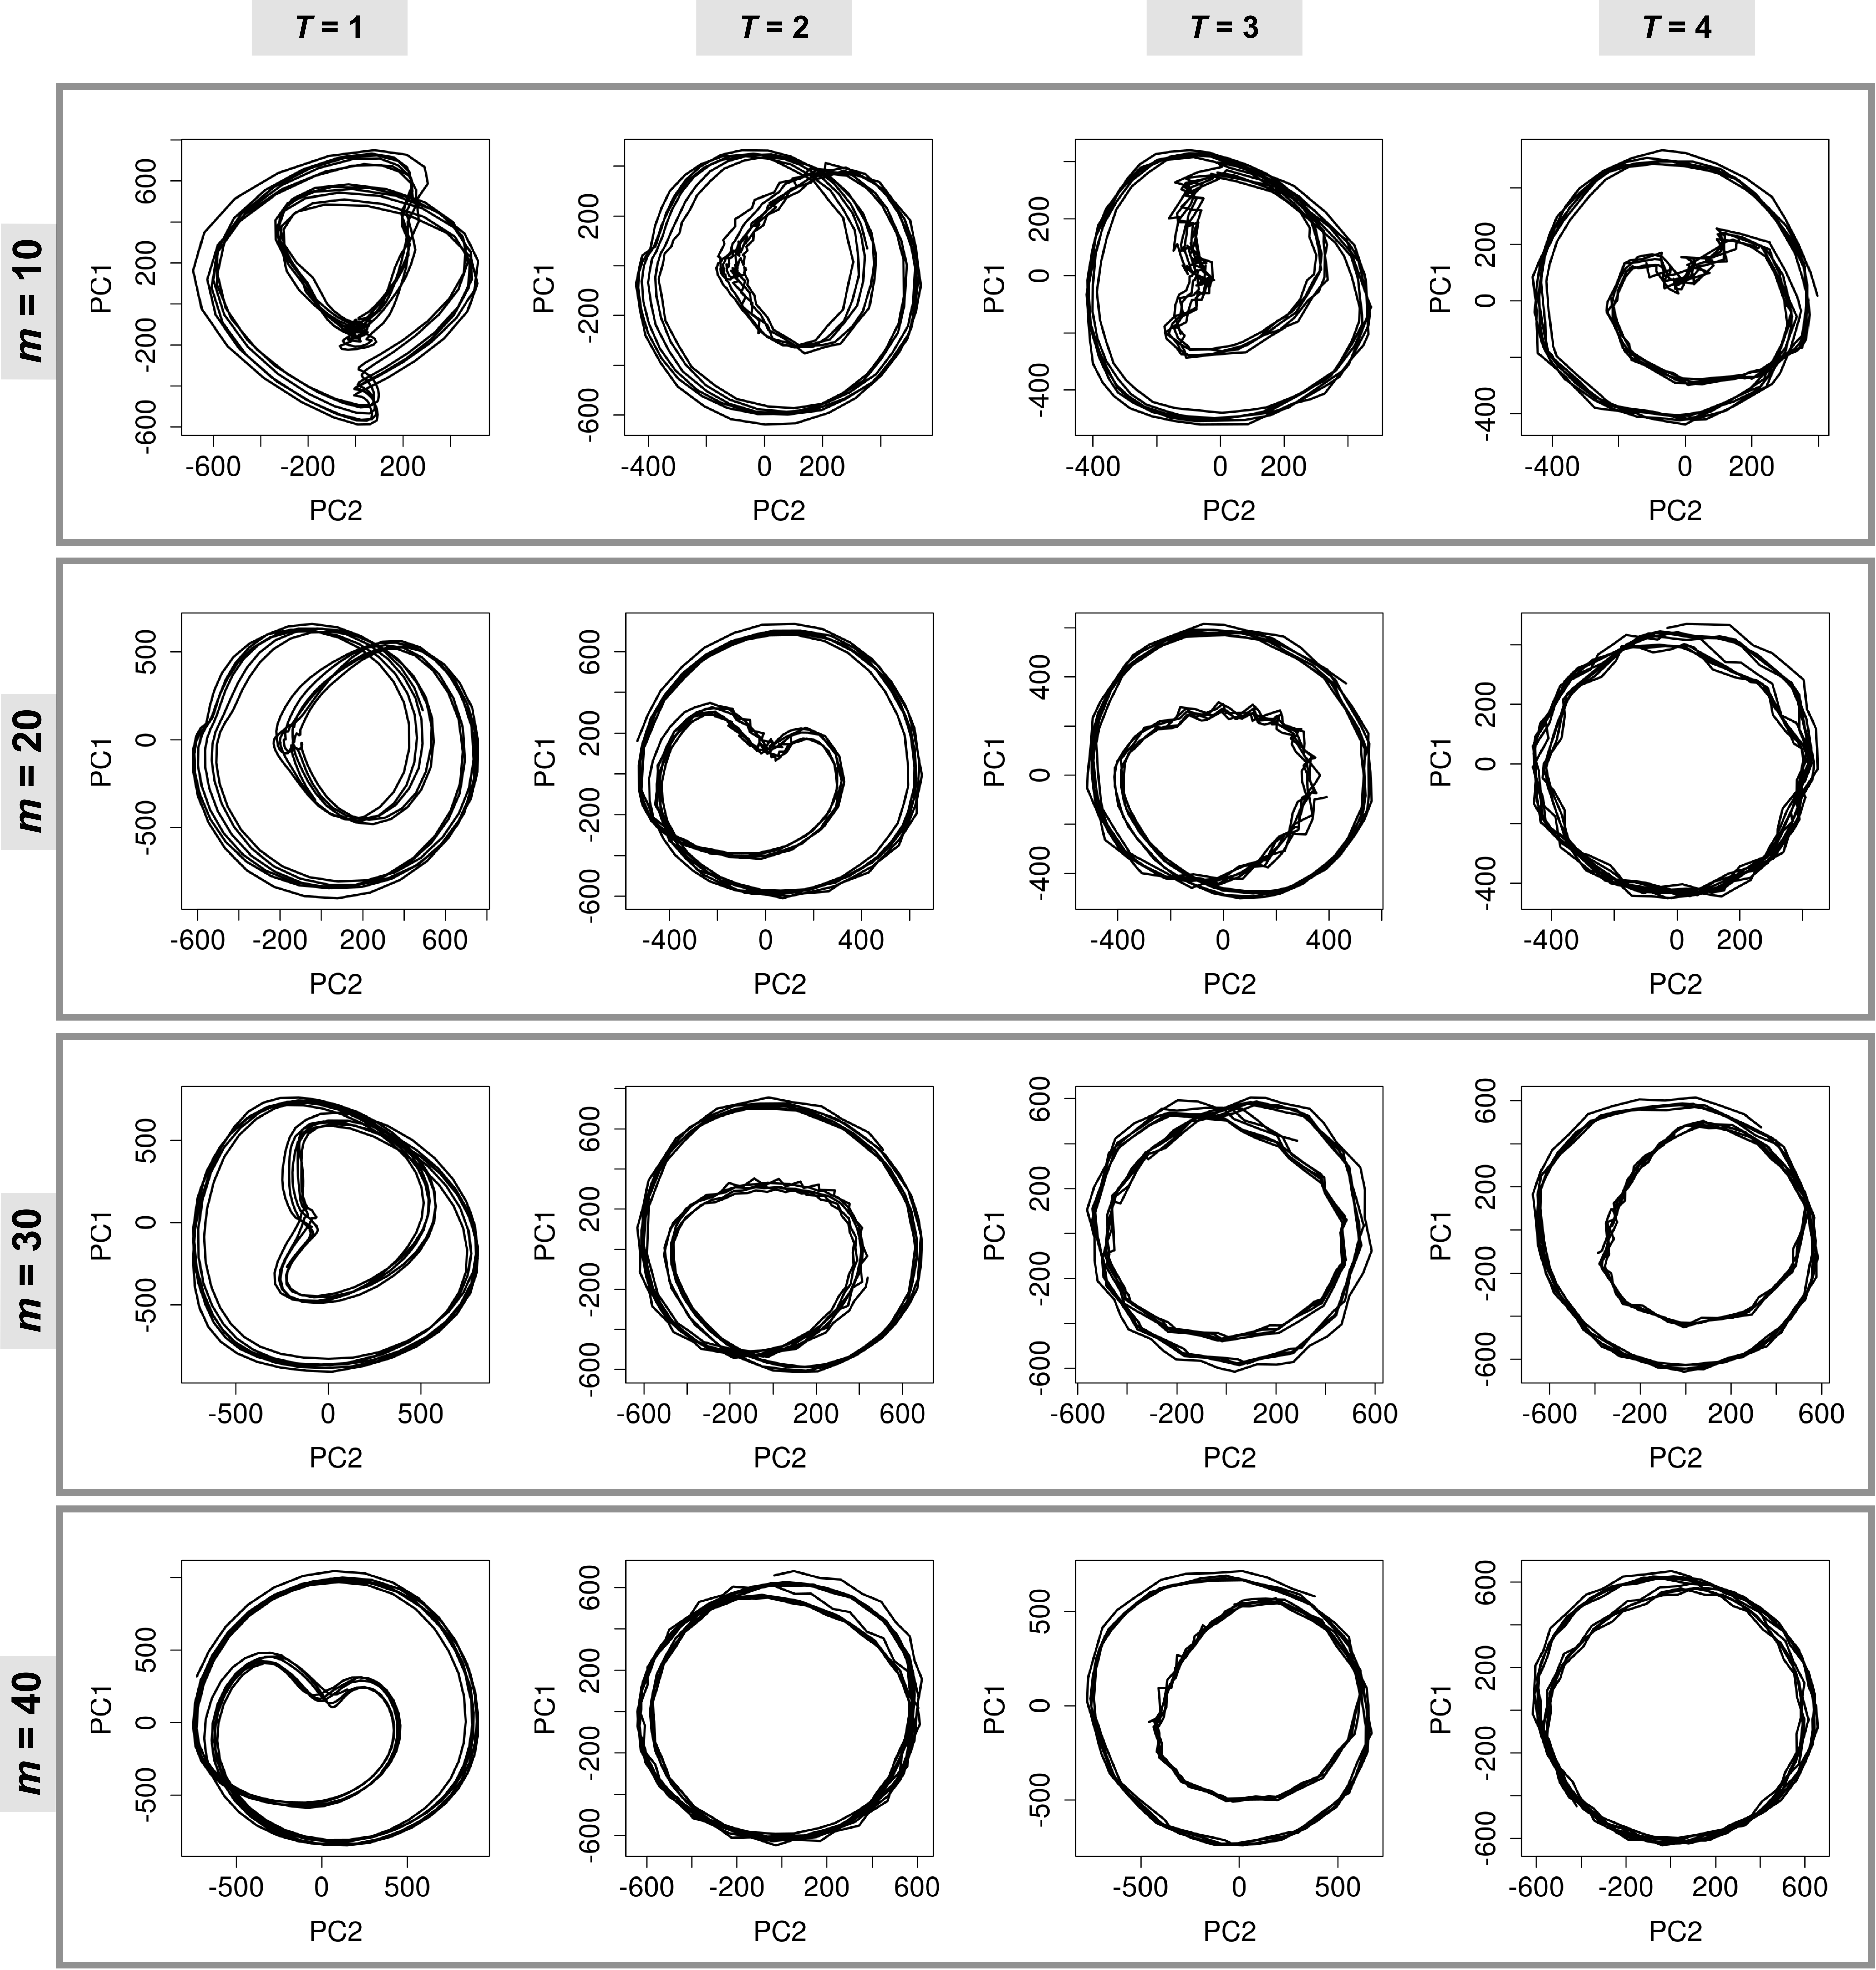
\includegraphics[width=0.45\textwidth]{takens}
\caption[PA]{2-D reconstructed state spaces with different embedded parameters 
($m=10,20,30,40$ and $\tau= 1,2,3,4$) for the expert dancing step 1.}
\label{fig:takens_problem}
\end{figure}








\section{Publication Plan}
Preliminary results were submitted to the International 
Symposium on Wearable Computers (ISWC) 2016; however, 
the submission was rejected because the reviewers argued 
that the method of using time-delay embedding and PCA
to quantify dexterity for salsa dancers is too specific and
it is not transferable to other applications. Additionally, 
they pointed out that data analysis were collected from 
11 novices, 1 intermediate and 1 expert dancers, and no 
classification framework was performed. 

I am planning to revise the ISWC paper to submit it in 
two possible conferences: Measuring Behaviour 2016 and
Augmented Human 2016.




\section{Future Work} 

To raise the bar in the field of human activity recognition,
the plan for the next six months is:
\begin{itemize}
\item \textbf{Aug. 2015 (10th)} Collect more data from experts 
  dancers so as to capture as much of the variability 
  as possible in either different dancers as well as 
  different dancing tasks.
\item \textbf{Sep. 2015 (11th)} Using the sawing data, present 
  the limitations of time-delay embedding and PCA 
  and propose improvements for the method. I am 
  also planning to investigate other non-linear analysis 
  tools that would be suitable to explore the variability 
  of dance activities.
\item \textbf{Oct. 2015 (12th)} Work towards a submission in 
  Measuring Behaviour 2016 and Augmented Human 
  2016 conferences.
\item \textbf{Nov. 2015 (13th)} Submit works in the Measuring 
  Behaviour 2016 and Augmented Human 2016 
  conferences.
\item \textbf{Dec. 2015 (14th)} Search for an appropriate journal 
  and work towards a submission.
\item \textbf{Jan. 2016 (15th)} Submit a journal publication
\end{itemize}







% use section* for acknowledgment
\ifCLASSOPTIONcompsoc
  % The Computer Society usually uses the plural form
  \section*{Acknowledgments}
\else
  % regular IEEE prefers the singular form
  \section*{Acknowledgment}
\fi

Miguel Xochicale gratefully acknowledges the studentship from 
the National Council for Science and Technology (CONACyT) Mexico
to pursue his postgraduate studies at University of Birmingham U.K.

\ifCLASSOPTIONcaptionsoff
  \newpage
\fi



% trigger a \newpage just before the given reference
% number - used to balance the columns on the last page
% adjust value as needed - may need to be readjusted if
% the document is modified later
%\IEEEtriggeratref{8}
% The "triggered" command can be changed if desired:
%\IEEEtriggercmd{\enlargethispage{-5in}}

% references section

% can use a bibliography generated by BibTeX as a .bbl file
% BibTeX documentation can be easily obtained at:
% http://www.ctan.org/tex-archive/biblio/bibtex/contrib/doc/
% The IEEEtran BibTeX style support page is at:
% http://www.michaelshell.org/tex/ieeetran/bibtex/
%\bibliographystyle{IEEEtran}
% argument is your BibTeX string definitions and bibliography database(s)
%\bibliography{IEEEabrv,../bib/paper}
%
% <OR> manually copy in the resultant .bbl file
% set second argument of \begin to the number of references
% (used to reserve space for the reference number labels box)
% \begin{thebibliography}{1}
% 
% \bibitem{IEEEhowto:kopka}
% H.~Kopka and P.~W. Daly, \emph{A Guide to \LaTeX}, 3rd~ed.\hskip 1em plus
%   0.5em minus 0.4em\relax Harlow, England: Addison-Wesley, 1999.
% 
% \end{thebibliography}

% \nocite{*}
\bibliographystyle{IEEEtran}
\bibliography{references}


% biography section
% 
% If you have an EPS/PDF photo (graphicx package needed) extra braces are
% needed around the contents of the optional argument to biography to prevent
% the LaTeX parser from getting confused when it sees the complicated
% \includegraphics command within an optional argument. (You could create
% your own custom macro containing the \includegraphics command to make things
% simpler here.)
%\begin{IEEEbiography}[{\includegraphics[width=1in,height=1.25in,clip,keepaspectratio]{mshell}}]{Michael Shell}
% or if you just want to reserve a space for a photo:

% \begin{IEEEbiography}[{\includegraphics[width=1in,height=1.25in,clip,keepaspectratio]{mxochicale38x44.pdf}}]{name}

% \begin{IEEEbiography}{Miguel Perez-Xochicale}
% ........................
% \end{IEEEbiography}



% % if you will not have a photo at all:
% \begin{IEEEbiographynophoto}{John Doe}
% Biography text here.
% \end{IEEEbiographynophoto}
% 
% % insert where needed to balance the two columns on the last page with
% % biographies
% %\newpage
% 
% \begin{IEEEbiographynophoto}{Jane Doe}
% Biography text here.
% \end{IEEEbiographynophoto}

% You can push biographies down or up by placing
% a \vfill before or after them. The appropriate
% use of \vfill depends on what kind of text is
% on the last page and whether or not the columns
% are being equalized.

%\vfill

% Can be used to pull up biographies so that the bottom of the last one
% is flush with the other column.
%\enlargethispage{-5in}



% that's all folks
\end{document}
